\chapter{Funciones}

\section{Las funciones y sus gráficas}

    %--------------------definición 1.1.
    \begin{tcolorbox}[colframe=white]
	\begin{def.}
	    Una función $f$ de un conjunto $D$ a un conjunto $Y$ es una regla que asigna a cada elemento $x \in D$ un solo o único elemento $f(x) \in Y$\\
	\end{def.}
    \end{tcolorbox}

    %--------------------definición 1.2.
    \begin{tcolorbox}[colframe=white]
	\begin{def.}
	    Cuando definimos una función $y = f(x)$ mediante una fórmula, y el dominio no se establece de forma explícita o se restringe por el contexto, se supondrá que el dominio será el mayor conjunto de números reales $x$ para los cuales la fórmula proporciona valores reales para $y$ , el llamado \textbf{dominio natural}.\\\\
	    Cuando el rango de una función es un subconjunto de números reales, se dice que la función tiene \textbf{valores reales (o que es real valuada)}\\
	\end{def.}
    \end{tcolorbox}

    %--------------------definición 1.3.
    \begin{tcolorbox}[colframe=white]
	\begin{def.}[Valor absoluto]
	    $f(x)=\left\{\begin{array}{rcl}
		x&si&x\geq 0\\
		\\ -x&si&x<0\\
	    \end{array} \right.$
	\end{def.}
    \end{tcolorbox}

    %--------------------definición 1.4.
    \begin{tcolorbox}[colframe=white]
	\begin{def.}
	    Sea una funcion definida en un intervalo $I$ y sean $x_1$ y $x_2$ cualesquiera dos puntos en $I$ 
	    \begin{enumerate}[\bfseries 1.]
		\item Si $f(x_2) > f(x_1)$, siempre que $x_1<x_2$ entonces se dice que $f$ es \textbf{creciente} en $I$.
		\item Si $f(x_2) < f(x_1)$, siempre que $x_1<x_2$ entonces se dice que $f$ es $\textbf{decreciente}$ en $I$.\\
	    \end{enumerate}
	\end{def.}
    \end{tcolorbox}

    %--------------------definición 1.5.
    \begin{tcolorbox}[colframe=white]
	\begin{def.}
	Una función $y=f(x)$ es una 
	    \begin{enumerate}[\bfseries 1.]
		\item Función par de $x$ si $f(-x)=f(x)$.
		\item Función impar de $x$ si $f(-x)=-f(x)$.
	    \end{enumerate}
	Para toda $x$ en el dominio de la función.\\\\
	(Los nombres par e impar provienen de las potencias de $x$).\\
	\end{def.}
    \end{tcolorbox}

    %--------------------definición 1.6.
    \begin{tcolorbox}[colframe=white]
	\begin{def.}
	    Dos variables $x$ e $y$ son \textbf{proporcionales} (una con respecto a la otra) si una siempre es un múltiplo constante de la otra; esto es, si $y=kx$ para alguna constante $k$ distinta de $0$.\\\\
	    Si la variable $y$ es proporcional al recíproco $1/x$, entonces algunas veces se dice que $y$ es \textbf{inversamente proporcional} a $x$ (puesto que $1/x$ es el inverso multiplicativo de $x$).\\

	\end{def.}
    \end{tcolorbox}


\setcounter{section}{0}
\section{Ejercicios}

\begin{enumerate}[\Large \bfseries 1.]

    %--------------------1.
    \item $f(x)=1+x^2$ \\\\
	Respuesta.-\; Al evaluar $1+x^2$ vemos que $x$ se cumple para todos los reales, por lo tanto $f_D=\lbrace x / \; \forall \; x \in \mathbb{R} \rbrace$. Luego el rango viene dado por $f_R=\lbrace y=f(x) / y \geq 1 \rbrace$\\\\

    %--------------------2.
    \item $f(x)=1-\sqrt{x}$\\\\
       Respuesta.-\; El dominio viene dado por $f_D=\lbrace x / x \geq 0 \rbrace$. Y el rango viene dado por $f_R = \lbrace y = f(x) / y \leq 1 \rbrace$.\\\\

    %--------------------3.
    \item $F(x)=\sqrt{5x + 10}$\\\\
	Respuesta.-\; Sea $5x + 10 \geq 0$ ya que una raíz par no puede ser no negativo, entonces $x \geq 2$, por lo tanto el dominio viene dado por $f_D=\lbrace x / x \geq -2 \rbrace$. Luego el rango viene dado por $f_R = \lbrace y=f(x) / y \geq 0 \rbrace$.\\\\

    %--------------------4.
    \item $g(x)=\sqrt{x^2 - 3x}$\\\\
	Respuesta.-\; De igual forma al anterior ejercicio, evaluaremos $x^2 - 3x \geq 0$, de donde $x(x-3)\geq 0$, por lo tanto el dominio es $f_D=\lbrace x/\leq x \leq 0 \cup x \geq 3 \rbrace$. Luego el rango viene definido por $f_R=\lbrace y=f(x) / y \geq 0 \rbrace$.\\\\

    %--------------------5.
    \item $f(t)=\dfrac{4}{3-t}$ \\\\
	Respuesta.-\; Sabemos que no se puede dividir un número por $0$. Por lo tanto para hallar el dominio de la función debemos evaluar $3-t=0$, de donde $t=3$, así $f_D=\lbrace t / t\neq 3\rbrace$. Luego el rango viene dado por $f_R=\lbrace y=f(x) / y\neq 0\rbrace$.\\\\

    %--------------------6.
    \item $G(t)=\dfrac{2}{t^2 - 16}$ \\\\
	Respuesta.-\; De igual forma al anterior ejercicio evaluamos $t^2 - 16 = 0$, de donde $(t - 4)(t + 4)=0$, por lo tanto el dominio de la función viene dado por $f_D=\lbrace t / t \neq 4 \land t \neq -4 \rbrace$. Luego el rango viene dado por $f_R=\lbrace y=f(x) / 0 < y \leq - \dfrac{1}{8} \rbrace$ ya que al despejar $x$ nos queda  $x=\sqrt{\dfrac{2}{y} + 16}$ de donde se debe evaluar por un lado $\dfrac{2}{y}$ y por otro $\dfrac{2}{y} - 16 \geq 0$.\\\\

    En los ejercicios $7$ y $8$ ¿Cuál de las gráficas representa la gráfica de una función de $x$? ¿Cuáles no representan a funciones de $x$? Dé razones que apoyen sus respuestas.\\\\

    %--------------------7.
    \item El inciso $a.$ no es una función ya que no cumple con la prueba de la recta vertical ya una función sólo puede tener un valor $f(x)$ para cada $x$ en su dominio. Y el inciso $b.$ no representa la gráfica de una función.\\\\

    %--------------------8.
    \item Los incisos $a.$ y $b.$ no representan a funciones de $x$. El único que no representa una gráfica de una función es el inciso $b.$\\\\

    Determinación de fórmulas para funciones.\\\\

    %--------------------9.
    \item Exprese el área y el perímetro de un triángulo equilátero como una función del lado $x$ del triángulo.\\\\
	Respuesta.-\; El área se representa por $f(x)=\dfrac{\sqrt{3}a^2}{4}$ y el perímetro por $f(x)=3x$\\\\

    %--------------------10.
    \item Exprese la longitud del lado de un cuadrado como una función de la longitud $d$ de la diagonal del cuadrado. Exprese el área como una función de la longitud de la diagonal.\\\\
	Respuesta.-\; La longitud del lado de un cuadrado como función de longitud esta dado por $d=\sqrt{2a^2}$. El área es expresado por $A=\dfrac{d^2}{2}$\\\\

    %--------------------11.
    \item Exprese la longitud del lado de um cubo como una función de la longitud de la diagonal $d$ del cubo. Exprese el área de la superficie y el volumen del cubo como una función de la longitud de la diagonal.\\\\
	Respuesta-.\; La expresión de la longitud del lado del cubo como función de la longitud de la diagonal $d$ del cubo es  $$ L(d) = (\sqrt{2}/2)\cdot d $$ 
	Las expresiones del área de la superficie y el volumen del cubo como función de la longitud de la diagonal $d$ del cubo son:
	$$A(d) = 3\cdot d^2 \quad    y \quad  V(d) = (\sqrt{2}/4)\cdot d^3$$

    %--------------------12.
    \item Un punto $P$ en el primer cuadrante pertenece a la gráfica de la función $f(x)=\sqrt{x}$. Exprese las coordenadas de $P$ como funciones de la pendiente de la recta que une a $P$ con el origen.\\\\
	Respuesta.-\; Sea el punto en el origen $(0,0)$ y el punto $P$ tenga las coordenadas $(z,z^{'})$. Sabemos que una recta viene definido por $f(x)=ax+b$ entonces formando un sistema de ecuaciones tenemos:
	$$0=0x + b \quad y \quad z^{'} = az + b$$
	Luego $z^{'}=az$ de donde $a=\dfrac{z^{'}}{z}$, y así nos queda la función  
	$$f(x)=\dfrac{z^{'}}{z} x$$\\\\

    %--------------------13.
    \item Considere el punto $(x,y)$ que está en la gráfica de la recta $2x + 4y = 5$. Sea $L$ la distancia del punto $(x, y)$ al origen $(0, 0)$. Escriba $L$ como función de $x$.\\\\
	Respuesta.-\; Dado $(x,y) \in 2x+4y=5 ; (0,0)$ entonces $$x=\dfrac{5-4y}{2} \qquad \dfrac{5-2x}{4}$$
	Luego $L=\sqrt{(y-0)^2+(x-0)^2} = \sqrt{y^2 + \left( \dfrac{5-4y}{2}\right)}=\sqrt{y^2 + \dfrac{25+40y+16y^2}{4}}=\sqrt{\dfrac{4y^2}{4} + \dfrac{25 - 40y + 16y^2}{4}} = \dfrac{1}{2} \sqrt{20y^2 + 40y + 25}$\\\\
 
    %--------------------14.
    \item Considere el punto $(x, y)$ que está en la gráfica de $y = \sqrt{x - 3}$. Sea $L$ la distancia entre los puntos $(x,y)$ y $(4,0)$. Escriba $L$ como función de $y$.\\\\
	Respuesta.-\; $y=\sqrt{x-3}, (x,y)\in y=\sqrt{x-3}$ entonces calculamos la distancia entre $y=\sqrt{x-3}$ y $(4,0)$.\\
	$$y^2=x-3 \Longrightarrow x=y^2 + 3 \quad y \quad y=\sqrt{x-3}$$ 
	Así $L=\sqrt{(y-o)^2 + (x-y)^2} = \sqrt{y^2 + (y^2 + 3)^2} = \sqrt{y^2 + y^4 + 6y^2 + 9} = \sqrt{y^4+7y^2+9}$\\\\

    Las funciones y sus gráficas.\\\\
    En los ejercicios $15$ al $20$, determine el dominio y grafique las funciones\\\\

    %--------------------15.
    \item $f(x)=5-2x$\\\\
	Respuesta.-\; El dominio esta dado para todos los reales $x$.
	\begin{center}
	    \begin{tikzpicture}[scale=1,draw opacity = 0.6]
		% abscisa y ordenada
		\tkzInit[xmax= 3,xmin=-2,ymax=5,ymin=-1]
		\tiny\tkzLabelXY[opacity=0.6,step=1, orig=false]
		% etiqueta x, f(x)
		\tkzDrawX[opacity=0.6,label=x,right=0.3]
		\tkzDrawY[opacity=0.6,label=f(x),below = -0.6]
		%dominio y función
		\draw [domain=-1:3,thick,gray] plot(\x,{5-2*\x});
		\tkzText[opacity=0.6,above](2,3){\tiny $f(x)=5-2x$}
	    \end{tikzpicture}
	\end{center}
	\vspace{.5cm}

    %--------------------16.
    \item $f(x)=1-2x-x^2$\\\\ 
	Respuesta.-\; El dominio viene dado para todo real $x$ positivo.
	\begin{center}
	    \begin{tikzpicture}[scale=1,draw opacity = 0.6]
		% abscisa y ordenada
		\tkzInit[xmax= 2,xmin=-3,ymax=3,ymin=-3]
		\tiny\tkzLabelXY[opacity=0.6,step=1, orig=false]
		% etiqueta x, f(x)
		\tkzDrawX[opacity=0.6,label=x,right=0.3]
		\tkzDrawY[opacity=0.6,label=f(x),below = -0.6]
		%dominio y función
		\draw [domain=-3:1,thick,gray] plot(\x,{1-2*\x - \x*\x});
		\tkzText[opacity=0.6,above](1.3,1){\tiny $f(x)=1-2x-x^2$}
	    \end{tikzpicture}
	\end{center}
	\vspace{.5cm}

    %--------------------17.
    \item $g(x)=\sqrt{|x|}$\\\\ 
	Respuesta.-\; El dominio de la función es para $x \in \mathbb{R}$
	\begin{center}
	    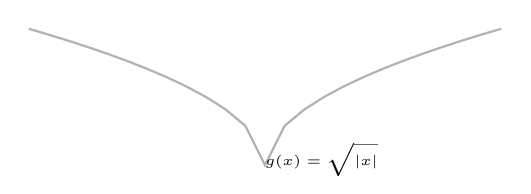
\begin{tikzpicture}[scale=1,draw opacity = 0.6]
		% abscisa y ordenada
		\tkzInit[xmax= 3,xmin=-3,ymax=3,ymin=0]
		\tiny\tkzLabelXY[opacity=0.6,step=1, orig=false]
		% etiqueta x, f(x)
		\tkzDrawX[opacity=0.6,label=x,right=0.3]
		\tkzDrawY[opacity=0.6,label=f(x),below = -0.6]
		%dominio y función
		\draw [domain=-3:3,thick,gray] plot(\x,{abs(\x)^(1/2)});
		\tkzText[opacity=0.6,above](1,1.7){\tiny $g(x)=\sqrt{|x|}$}
	    \end{tikzpicture}
	\end{center}
	\vspace{.5cm}

    %--------------------18.
    \item $g(x) = \sqrt{-x}$\\\\
	Respuesta.-\; El dominio de la función se cumple para los números reales negativos.   
	\begin{center}
	    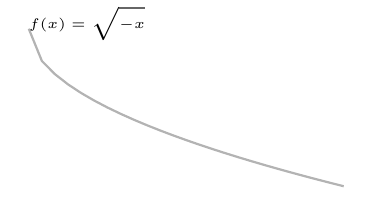
\begin{tikzpicture}[scale=1,draw opacity = 0.6]
		% abscisa y ordenada
		\tkzInit[xmax= 4,xmin=-1,ymax=1,ymin=-2]
		\tiny\tkzLabelXY[opacity=0.6,step=1, orig=false]
		% etiqueta x, f(x)
		\tkzDrawX[opacity=0.6,label=x,right=0.3]
		\tkzDrawY[opacity=0.6,label=f(x),below = -0.6]
		%dominio y función
		\draw [domain=0:4,thick,gray] plot(\x,{-\x^(1/2)});
		\tkzText[opacity=0.6,above](2,-1){\tiny $f(x)=\sqrt{-x}$}
	    \end{tikzpicture}
	\end{center}
	\vspace{.5cm}

    %--------------------19.
    \item $F(t)=t/|t|$\\\\
	Respuesta.-\; El dominio viene dado para todo número real menos el $0$. 
	\begin{center}
	    \begin{tikzpicture}[scale=1,draw opacity = 0.6]
		% abscisa y ordenada
		\tkzInit[xmax= 3,xmin=-3,ymax=2,ymin=-2]
		\tiny\tkzLabelXY[opacity=0.6,step=1, orig=false]
		% etiqueta x, f(x)
		\tkzDrawX[opacity=0.6,label=x,right=0.3]
		\tkzDrawY[opacity=0.6,label=f(x),below = -0.6]
		%dominio y función
		\draw [domain=.1:3,thick,gray] plot(\x,{\x/abs(\x)});
		\draw [domain=-3:-.1,thick,gray] plot(\x,{\x/abs(\x)});
		\tkzText[opacity=0.6,above](1,1){\tiny $F(t)=t/|t|$}
	    \end{tikzpicture}
	\end{center}
	\vspace{.5cm}

    %--------------------20.
    \item $G(t)=1/|t|$\\\\
	Respuesta.-\; El dominio se cumple para todo número real menos el $0$.
	\begin{center}
	    \begin{tikzpicture}[scale=1,draw opacity = 0.6]
		% abscisa y ordenada
		\tkzInit[xmax= 3,xmin=-3,ymax=5,ymin=0]
		\tiny\tkzLabelXY[opacity=0.6,step=1, orig=false]
		% etiqueta x, f(x)
		\tkzDrawX[opacity=0.6,label=x,right=0.3]
		\tkzDrawY[opacity=0.6,label=f(x),below = -0.6]
		%dominio y función
		\draw [domain=.2:3,thick,gray] plot(\x,{1/abs(\x)});
		\draw [domain=-3:-.2,thick,gray] plot(\x,{1/abs(\x)});
		\tkzText[opacity=0.6,above](2,2){\tiny $G(t)=1/|t|$}
	    \end{tikzpicture}
	\end{center}
	\vspace{.5cm}

    %--------------------21
    \item Determine el dominio de $y=\dfrac{x+3}{4-\sqrt{x^2-9}}$\\\\
	Respuesta.-\; Si $y=f(x)$ entonces el dominio esta dado por $D_f=\lbrace x / x\geq 3 \land x \neq 4 \rbrace$ \\\\

    %--------------------22.
    \item Determine el rango de $y=2+\dfrac{x^2}{x^2+4}$.\\\\
	Respuesta.-\; Si $y=f(x)$ entonces el rango viene dado para todo $y=f(x)$ tal que $y\geq 2$\\\\

    %--------------------23.
    \item Grafique las siguientes ecuaciones y explique por qué no son gráficas de funciones de $x$.\\\\
    
    \begin{enumerate}[\bfseries a.]
	
	%----------a.
	\item $|y|=x$\\\\
	    Respuesta.-\; No es una función de $x$ ya que $ \sqrt{y^2}=x \Longrightarrow y^2=x^2 \Longrightarrow \pm y = \pm x$\\\\

	%----------b.
	\item $y^2 = x^2$\\\\
	    Respuesta.-\; Por el anterior problema $23a.$\\\\
	
    \end{enumerate}

    %--------------------24.
    \item Grafique las siguientes ecuaciones y explique por qué no son gráficas de funciones de $x$\\\\

    \begin{enumerate}[\bfseries a.]

	%----------a.
	\item $|x|+|y|=1$\\\\
	    Respuesta.-\; Ya que $|y|=1 - |x| \Longrightarrow \sqrt{y^2} = 1 - |x| \Longrightarrow y^2 = (1-|x|)^2 \Longrightarrow \pm y= |1-|x||$\\\\

	%----------b.
	\item $|x+y|=1$\\\\
	Respuesta.-\;  Ya que $\sqrt{(x+y)^2}=1 \Longrightarrow (x+y)^2 = 1 \Longrightarrow x^2 + 2xy + y^2 = 1 \Longrightarrow y^2 = 1 - 2xy - x^2 \Longrightarrow \pm y = \sqrt{1-2xy-x^2}$\\\\
    \end{enumerate}

    Funciones definidas por partes\\\\
    En los ejercicios 25 a 28, grafique las funciones:\\\\

    %--------------------25.
    \item $f(x) = \left\{ \begin{array}{cc}
		    x,&0\leq x \leq 1\\
		    \\ 2-x,&1<x\leq 2 \\
		    \end{array} \right.$
	\begin{center}
	    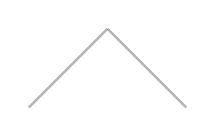
\begin{tikzpicture}[scale=1,draw opacity = 0.6]
		% abscisa y ordenada
		\tkzInit[xmax= 3,xmin=-1,ymax=2,ymin=0]
		\tiny\tkzLabelXY[opacity=0.6,step=1, orig=false]
		% etiqueta x, f(x)
		\tkzDrawX[opacity=0.6,label=x,right=0.3]
		\tkzDrawY[opacity=0.6,label=f(x),below = -0.6]
		%dominio y función
		\draw [domain=0:1,thick,gray] plot(\x,{\x});
		\draw [domain=1:2,thick,gray] plot(\x,{2-\x});
	    \end{tikzpicture}
	\end{center}
	\vspace{.5cm}
    
    %--------------------26.
    \item $g(x) = \left\{ \begin{array}{cc}
		    1-x,&0\leq x \leq 1\\
		    \\ 2-x,&1<x\leq 2 \\
		    \end{array} \right.$
	\begin{center}
	    
\begin{tikzpicture}[scale=1,draw opacity = 0.6]
		% abscisa y ordenada
		\tkzInit[xmax= 3,xmin=-1,ymax=2,ymin=0]
		\tiny\tkzLabelXY[opacity=0.6,step=1, orig=false]
		% etiqueta x, f(x)
		\tkzDrawX[opacity=0.6,label=x,right=0.3]
		\tkzDrawY[opacity=0.6,label=f(x),below = -0.6]
		%dominio y función
		\draw [domain=0:1,thick,gray] plot(\x,{1-\x});
		\draw [domain=1:2,thick,gray] plot(\x,{2-\x});
	    \end{tikzpicture}
	\end{center}
	\vspace{.5cm}
    
    %--------------------27.
    \item $F(x) = \left\{ \begin{array}{cc}
		    4-x^2,&\leq 1 \\
		    \\ x^2 + 2x,& x>1 \\
		    \end{array} \right.$
	\begin{center}
	    \begin{tikzpicture}[scale=1,draw opacity = 0.6]
		% abscisa y ordenada
		\tkzInit[xmax= 3,xmin=-3,ymax=8,ymin=0]
		\tiny\tkzLabelXY[opacity=0.6,step=1, orig=false]
		% etiqueta x, f(x)
		\tkzDrawX[opacity=0.6,label=x,right=0.3]
		\tkzDrawY[opacity=0.6,label=f(x),below = -0.6]
		%dominio y función
		\draw [domain=-2:1,thick,gray] plot(\x,{4-\x*\x});
		\draw [domain=1:2,thick,gray] plot(\x,{\x*\x + 2*\x});
	    \end{tikzpicture}
	\end{center}
	\vspace{.5cm}

    %--------------------28.
    \item $G(x) = \left\{ \begin{array}{cc}
		    1/x,&x<0\\
		    \\ x, & 0\leq x \\
		    \end{array} \right.$
	\begin{center}
	    \begin{tikzpicture}[scale=1,draw opacity = 0.6]
		% abscisa y ordenada
		\tkzInit[xmax= 3,xmin=-4,ymax=2,ymin=-8]
		\tiny\tkzLabelXY[opacity=0.6,step=1, orig=false]
		% etiqueta x, f(x)
		\tkzDrawX[opacity=0.6,label=x,right=0.3]
		\tkzDrawY[opacity=0.6,label=f(x),below = -0.6]
		%dominio y función
		\draw [domain=-3:0,thick,gray] plot(\x,{1*\x^(-1)});
		\draw [domain=0:2,thick,gray] plot(\x,{\x});
	    \end{tikzpicture}
	\end{center}
	\vspace{.5cm}

    Determine una fórmula para cada función graficada en los ejercicios $29$ a $32$\\\\

    %--------------------29
    \item 
    \begin{enumerate}[\bfseries a.]
	
	%----------a.
	\item  Sea $f(x)=ax+b$ entonces $0=b$ y $1=a+b$ luego $a=1$ por lo tanto $f(x)=x$. Por otro lado $1=a+b$ y $0=2a+2 \Longrightarrow a=-1$ de donde se tiene $f(x^{'})=-x+2$ así nos queda la función:
	$$f(x) = \left\{\begin{array}{r c l}
		x&si&0\leq x \leq 1\\
		\\ x+2&si&1\leq x \leq 2 \\
	    \end{array}\right.$$\\\\

	%----------b.
	\item Está definida por $$f(x)=\left\{\begin{array}{rcl} 
				    2&si&0\leq x < 1 \; y \; 2 \leq x < 3\\
				    \\  0&si& 1\leq x < 2 \; y \; 3\leq x \leq 4\\
				    \end{array}\right.$$\\\\

    \end{enumerate}

    %--------------------30.
    \item 
    \begin{enumerate}[\bfseries a.]

	%----------a.
	\item Similar al ejercicio anterior se tiene que la formula 
	$$f(x)= \left\{ \begin{array}{rcl}
		x+2&si& 0 \leq x \leq 2 \\
		\\ 1/2x+5/7&si& 0\leq x \leq 2 \\ \end{array}\right.$$\\\\

	%----------b.
	\item Se tiene 
	$$f(x)=\left\{\begin{array}{rcl} 
		-3x - 3&si&-1\leq x \leq 0\\
		\\-2x + 3&si&\\ \end{array} \right.$$\\\\

    \end{enumerate}

    %--------------------31.
    \item 
    \begin{enumerate}[\bfseries a.]

	%----------a.
	\item  
	$$f(x)= \left\{ \begin{array}{rcl}
		x+2&si& -1 \leq x < 0 \\
		\\ 1&si& 0 < x \leq 1 \\ 
		\\ -2x + 2&si&1 \leq x \leq 3\\
		\end{array}\right.$$\\\\
	
	%----------b.
	\item Sea $(a,b)$ y $(c,d)$ por lo tanto por capitulo $4$ de spivak $f(x)=\dfrac{d-b}{c-a}(x-a)+b$ entonces $(-2,-1)$ y $(0,0)$ así $f(x)=\dfrac{0-1}{0+2}(x+2) + 0 \quad \Longrightarrow \quad f(x) = -\dfrac{1}{2}x - 2$ \\\\
	Luego $f(x)=-2x+2$ y finalmente $f(x)=-1$ de donde,
	$$f(x)= \left\{ \begin{array}{rcl}
		- \dfrac{1}{2}x -2&si& -2 \leq x \leq 0 \\
		\\ 2x+2&si& 0 < x \leq 1 \\ 
		\\ -1&si&1 < x \leq 3\\
		\end{array}\right.$$\\\\
    \end{enumerate}

    %--------------------32.
    \item 
    \begin{enumerate}[\bfseries a.]

	%----------a.
	\item 
	$$f(x)= \left\{ \begin{array}{rcl}
		0&si& 0 \leq x \leq \dfrac{T}{2} \\\\
		\\ \dfrac{2x}{T} - 1&si& \dfrac{T}{2}< x \leq T \\\\ 
		\end{array}\right.$$\\\\

	%----------b.
	\item  
	$$f(x)= \left\{ \begin{array}{rcl}
		A&si& \dfrac{T}{2} \leq x < T \quad y \quad T \leq x < \dfrac{3T}{2}\\\\
		\\ -A&si&\dfrac{T}{2} \leq x < T \quad y \quad \dfrac{3T}{2} \leq x \leq 2T \\\\
		\end{array}\right.$$\\\\

    \end{enumerate}

Las funciones mayor entero y menor entero.\\\\

    %--------------------33.
    \item Para qué valores de $x$ es 
    \begin{enumerate}[\bfseries a.]
	\item $[x]=0$\\\\
	    respuesta.-\; Para $0\leq x < 1$\\\\
	\item $[x] =0$\\\\
	    Respuesta.-\; Para $-1 < x \leq 0$\\\\
    \end{enumerate}

    %--------------------34.
    \item ¿Cuáles valores $x$ de números reales satisfacen la ecuación $[x] = [x]$?\\\\
	Respuesta.-\; Sólo el $0$.\\\\

    %--------------------35.
    \item ¿Es cierto que $[-x] = -[x]$ para todo número real $x$? Justifique su respuesta.\\\\
	Respuesta.-\; Es cierto siempre y cuando sea $x$ un entero. Ya que si $x\in \mathbb{Z}$ entonces $x=n$ para algunos $n\in \mathbb{Z}$, por lo tanto $[x]=n$ y $-x=-n \Longrightarrow [-x] = n \Longrightarrow [-x] = -[x]$. Por otro lado sea $x \notin \mathbb{Z}$ y $[x]=n$ entonces  $n\leq x < n+1 \Longrightarrow -n-1<-x<-n \Longrightarrow [-x] = -n-1 = -[x] - 1$\\\\

    %--------------------36.
	\item Grafique la función 
		$$f(x) = \left\{\begin{array}{cl}
			[x],&x\leq 0\\
			 x,&x<0\\
			\end{array}\right.$$ 
	    ¿Por qué $f(x)$ se donomina parte entera de $x$?\\\\
	    Respuesta.-\; Se denomia porque hace corresponder el número inmediato anterior.\\\\

    Funciones crecientes y funciones decrecientes.\\\\
    Grafique las funciones en los ejercicios 37 a 46. Si tiene simetrías, ¿Qué tipo de simetría tienen? Especifique los intervalos en os que la función es creciente y los intervalos donde la función es decreciente.\\\\ 

    %--------------------37
    \item $y=-x^3$
	\begin{center}
	    \begin{tikzpicture}[scale=1,draw opacity = 0.6]
		% abscisa y ordenada
		\tkzInit[xmax= 2,xmin=-2,ymax=2,ymin=-2.2]
		\tiny\tkzLabelXY[opacity=0.6,step=1, orig=false]
		% etiqueta x, f(x)
		\tkzDrawX[opacity=0.6,label=x,right=0.3]
		\tkzDrawY[opacity=0.6,label=f(x),below = -0.6]
		%dominio y función
		\draw [domain=-1.3:1.3,thick,gray] plot(\x,{-\x^3});
	    \end{tikzpicture}
	\end{center}
	\vspace{.5cm}
	Respuesta.-\; Tiene simetría impar y el intervalo donde decrece esta dado por $(-\infty,\infty)$\\\\

    %--------------------38.
    \item $y=-\dfrac{1}{x^2}$\\\\
	Respuesta.-\; Tiene simetría par y esta dado por lo el intervalo decreciente de $-\infty<x<0$ y por el intervalo creciente $0<x<\infty$

    %--------------------39.
    \item $y=-\dfrac{1}{x}$\\\\
	Respuesta.-\; Tiene simetría impar y viene dado por los intervalos crecientes $-\infty < x < 0$  y $0<x<\infty$\\\\

    %--------------------40.
    \item $y=\dfrac{1}{|x|}$\\\\
	Respuesta.-\; Tiene simetría par y viene dado por el intervalo creciente $-\infty<x<0$ y el intervalo decreciente $0<x<\infty$\\\\

    %--------------------41.
    \item $y=\sqrt{|x|}$\\\\
	\begin{center}
	    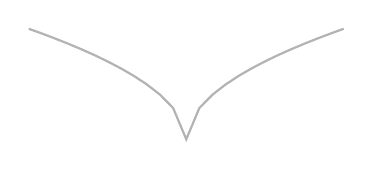
\begin{tikzpicture}[scale=1,draw opacity = 0.6]
		% abscisa y ordenada
		\tkzInit[xmax= 2,xmin=-2,ymax=2,ymin=0]
		\tiny\tkzLabelXY[opacity=0.6,step=1, orig=false]
		% etiqueta x, f(x)
		\tkzDrawX[opacity=0.6,label=x,right=0.3]
		\tkzDrawY[opacity=0.6,label=f(x),below = -0.6]
		%dominio y función
		\draw [domain=-2:2,thick,gray] plot(\x,{sqrt(abs(\x))});
	    \end{tikzpicture}
	\end{center}
	\vspace{.5cm}
	Respuesta.-\; Tiene simetría par y esta dado por el intervalo  decreciente  $-\infty < x \leq 0$ y el intervalo creciente $0\leq x < \infty$\\\\

    %--------------------42.
    \item $y=\sqrt{-x}$\\\\
	\begin{center}
	    \begin{tikzpicture}[scale=1,draw opacity = 0.6]
		% abscisa y ordenada
		\tkzInit[xmax= 2,xmin=-2,ymax=2,ymin=0]
		\tiny\tkzLabelXY[opacity=0.6,step=1, orig=false]
		% etiqueta x, f(x)
		\tkzDrawX[opacity=0.6,label=x,right=0.3]
		\tkzDrawY[opacity=0.6,label=f(x),below = -0.6]
		%dominio y función
		\draw [domain=-2:0,thick,gray] plot(\x,{sqrt(-\x)});
	    \end{tikzpicture}
	\end{center}
	\vspace{.5cm}
	Respuesta.- No es ni par ni impar y viene dado por el intervalo decreciente $-\infty < x \leq 0$\\\\

    %-------------------43.
    \item $y=x^3/8$\\\\
	\begin{center}
	    \begin{tikzpicture}[scale=1,draw opacity = 0.6]
		% abscisa y ordenada
		\tkzInit[xmax= 3,xmin=-3,ymax=2,ymin=-2]
		\tiny\tkzLabelXY[opacity=0.6,step=1, orig=false]
		% etiqueta x, f(x)
		\tkzDrawX[opacity=0.6,label=x,right=0.3]
		\tkzDrawY[opacity=0.6,label=f(x),below = -0.6]
		%dominio y función
		\draw [domain=-2.5:2.5,thick,gray] plot(\x,{\x^3/8});
	    \end{tikzpicture}
	\end{center}
	\vspace{.5cm}
	Respuesta.-\; Tiene simetría impar y viene dado por el intervalo creciente $-\infty < x < \infty$\\\\

    %---------------------44.
    \item $y=-4\sqrt{x}$\\\\
	\begin{center}
	    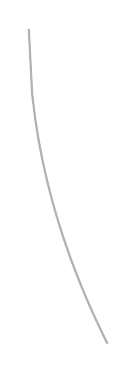
\begin{tikzpicture}[scale=1,draw opacity = 0.6]
		% abscisa y ordenada
		\tkzInit[xmax= 2,xmin=-1,ymax=1,ymin=-4]
		\tiny\tkzLabelXY[opacity=0.6,step=1, orig=false]
		% etiqueta x, f(x)
		\tkzDrawX[opacity=0.6,label=x,right=0.3]
		\tkzDrawY[opacity=0.6,label=f(x),below = -0.6]
		%dominio y función
		\draw [domain=0:1,thick,gray] plot(\x,{-4*sqrt(\x)});
	    \end{tikzpicture}
	\end{center}
	\vspace{.5cm}
	Respuesta.-\; No es ni par ni impar y viene dado por el intervalo $0\leq x < \infty$\\\\

    %--------------------45.
    \item $y=-x^{3/2}$\\\\
	\begin{center}
	    \begin{tikzpicture}[scale=1,draw opacity = 0.6]
		% abscisa y ordenada
		\tkzInit[xmax= 2,xmin=-1,ymax=1,ymin=-1]
		\tiny\tkzLabelXY[opacity=0.6,step=1, orig=false]
		% etiqueta x, f(x)
		\tkzDrawX[opacity=0.6,label=x,right=0.3]
		\tkzDrawY[opacity=0.6,label=f(x),below = -0.6]
		%dominio y función
		\draw [domain=-1:1,thick,gray] plot(\x,{-(\x^(3/2))});
	    \end{tikzpicture}
	\end{center}
	\vspace{.5cm}
	Respuesta.-\; Tiene simetría impar y viene dado por el intervalo decreciente $-\infty < x < \infty$\\\\

    %---------------------46.
    \item $y=(-x)^{2/3}$\\\\
	\begin{center}
	    \begin{tikzpicture}[scale=1,draw opacity = 0.6]
		% abscisa y ordenada
		\tkzInit[xmax= 2,xmin=-1,ymax=1,ymin=-1]
		\tiny\tkzLabelXY[opacity=0.6,step=1, orig=false]
		% etiqueta x, f(x)
		\tkzDrawX[opacity=0.6,label=x,right=0.3]
		\tkzDrawY[opacity=0.6,label=f(x),below = -0.6]
		%dominio y función
		\draw [domain=-1:1,thick,gray] plot(\x,{\x^(2/3)});
	    \end{tikzpicture}
	\end{center}
	\vspace{.5cm}
	Respuesta.-\; La simetría es impar y viene dado por el intervalo creciente $-\infty < x < \infty$\\\\

    Funciones pares y funciones impares \\\\
    En los ejercicios $47$ a $58$, indique si la función es par, impar o de ninguno de estos tipos. Justifique su respuesta.\\\\

    %--------------------47.
    \item $f(x)=3$\\\\
	Respuesta.-\; Sea $f(-x)=3=f(x)$ entonces decimos que la función es par.\\\\

    %--------------------48.
    \item $f(x)=x^{-5}$\\\\
	Respuesta.-\; Sea $f(-x)=(-x)^{-5} = -\left(x^{-5}\right)=-f(x)$, por lo tanto la función es impar.\\\\

    %--------------------49.
    \item $f(x)=x^2 + 1$\\\\
	Respuesta.-\; Sea $f(-x)=(-x)^2 + 1 = x^2 + 1 = f(x)$, de donde se tiene que la función es par.\\\\

    %--------------------50.
    \item $f(x)=x^2 + x$\\\\
	Respuesta.-\; Sea $f(-x)=(-x)^2 + (-x) = x^2 - x$ de donde la función no es par ni impar.\\\\

    %--------------------51.
    \item $g(x)=x^3  + x$\\\\
	Respuesta.-\; Sea $f(-x) = (-x)^3 + (-x) = -(x^3 + x) = -f(x)$ por lo tanto la función es impar.\\\\

    %--------------------52.
    \item $g(x)=x^4 + 3x^2 - 1$\\\\
	Respuesta.-\; Sea $g(-x) = (-x)^4 + 3(-x)^2 - 1 = g(x)$ por lo tanto la función es par.\\\\

    %--------------------53.
    \item $g(x)=\dfrac{1}{x^2-1}$\\\\
	Respuesta.-\; Sea $g(-x)=\dfrac{1}{(-x)^2 - 1} = g(x)$ por lo tanto la función es par.\\\\

    %--------------------54.
    \item $g(x)=\dfrac{x}{x^2 - 1}$\\\\
	Respuesta.-\; Sea $g(-x)=\dfrac{-x}{(-x)^2 - 1} = - \dfrac{x}{x^2 - 1} = -g(x)$ de donde la función es impar.\\\\

    %--------------------55.
    \item $h(t)=\dfrac{1}{t-1}$\\\\
	Respuesta.-\; Sea $h(-t)=\dfrac{1}{-t-1}$ entonces la función no es par ni impar.\\\\

    %--------------------56.
    \item $h(t)=|t^3|$\\\\
	Respuesta.-\; Sea $h(-t)=|(-t)^3| = |t^3| = h(t)$ por lo tanto la función es par.\\\\

    %--------------------57.
    \item $h(t)=2t+1$\\\\
	Respuesta.-\; Sea $h(-t) = 2(-t) + 1$ entonces la función no es ni par ni impar.\\\\

    %--------------------58.
    \item $h(t)=2|t|+1$\\\\
	Respuesta.-\; Sea $h(-t)=2|-t| + 1 = 2t + 1 = h(t)$ entonces la función es par.\\\\

    Teoría y ejemplos\\\\

    %--------------------59.
    \item La variable $s$ es proporcional a $t$, y $s=25$ cuando $t=75$. Determine $t$ cuando $s=60.$\\\\
	Respuesta.-\; Sea $\dfrac{s}{r}$ entonces $\dfrac{25}{75}=\dfrac{60}{x} \quad \Rightarrow \quad \dfrac{1}{3} = \dfrac{60}{x} \quad \Rightarrow \quad x=180$\\\\ 

    %--------------------60.
    \item Energía cinética. La energía cinética $K$ de una masa es proprocional al cuadrado de su velocidad $v$. Si $K=12,960$ joules, cuando $v=18$ m/s, ¿Cuál es el valor de $K$ cuando $v=10$ m/s?.\\\\
	Respuesta.-\; Similar al anterior ejercicio se tiene $\dfrac{K}{v^2} = \dfrac{12,960}{18^2} = \dfrac{K}{10^2}$ entonces $K=4000$.\\\\

    %--------------------61.
    \item Las variables $r$ y $s$ son inversamente proporcional, mientras que $r=6$ cuando $s=4$. Determine $s$ cuando $r=10$.\\\\
	Respuesta.-\; Tenemos que $6\cdot 4 = s \cdot 10$ entonces queda que $s = 2.4$.\\\\

    %--------------------62.
    \item Ley de Boyle. La ley de Boyle establece que el volumen $V$ de un gas, a temperatura constante, aumenta cuando la presión $P$ disminuye, de manera que $V$ y $P$ son inversamente proporcionales. Si $P = 14.7 lb/in^2$ cuando $V = 1000 in^3$, entonces ¿cuál es el valor de $V$ cuando $P = 23.4 lbs/in^2$?.\\\\
	Respuesta.-\; Sea $V\cdot P = V^{'} \cdot P^{'}$ entonces $14.7 \cdot 1000 = V \cdot 23.4$ y por lo tanto $V=628.2 in^3$.\\\\

    %--------------------63.
    \item Una caja sin tapa se construye a partir de una pieza rectangular de cartón, cuyas dimensiones son $14$ por $22$ pulgadas (in). A la pieza de cartón se le cortan cuadrados de lado $x$ en cada esquina y luego se doblan hacia arriba los lados, como en la figura. Exprese el volumen $V$ de la caja como una función de $x$.\\\\
	Respuesta.-\; El volumen es dado por $V=L\cdot a\cdot h$ luego $h=x,\qquad a=14-2x, \qquad L=22-2x$ por lo tanto $$V(x)=(22-2x)(14-2x)\cdot x \quad \Longrightarrow \quad V(x)=4x^3 - 72x^2 + 308x$$\\\\

    %--------------------64.
    \item La siguiente figura muestra un rectángulo inscrito en un triángulo rectángulo isósceles, cuya hipotenusa tiene una longitud de dos unidades.
    \begin{enumerate}[\bfseries a.]
	
	%----------a.
	\item Exprese la coordenada de $P$ en términos de $x$. (Podría iniciar escribiendo una ecuación para la recta $AB$).\\\\
	    Respuesta.-\; Sea $y=mx+b$ luego en el punto $B$, se tiene la intersección de ambas rectas que forman un ángulo de $90^{\circ}$, así que, el ángulo que tiene que tener el punto $A$ es de $45^{\circ}$ o bien $m=-1$ por lo tanto $y=-x+b$ o bien m=-1 ya que la recta va hacia abajo.\\\\

	%----------b.
	\item Exprese el área del rectángulo en términos de $x$.\\\\
	    Respuesta.-\; El área de un rectángulo es $b\cdot a$ de donde $area = 2x \cdot y = 2x(b-x)$.\\\\

    \end{enumerate}

    En los ejercicios 65 y 66 relacione cada ecuación con su gráfica. No utilice un dispositivo para graficar y dé razones que justifiquen su respuesta.\\\\

    %--------------------65.
    \item  
    \begin{enumerate}[\bfseries a.]
	
	%----------a.
	\item $y=x^4 \quad \Rightarrow \quad h$\\\\

	%----------b.
	\item $y=x^7 \quad  \Rightarrow \quad f$\\\\

	%----------c.
	\item $y=x^10 \quad \Rightarrow \quad g$\\\\

    \end{enumerate}

    %--------------------66.
    \item
    \begin{enumerate}[\bfseries a.]
	
	%----------a.
	\item $y=5x \quad \Rightarrow \quad f$.\\\\

	%----------b.
	\item $y=5x \quad \Rightarrow \quad f$.\\\\

	%----------c.
	\item $y=x^5 \quad \Rightarrow \quad h$.\\\\

    \end{enumerate}

    %--------------------67.
    \item 
    \begin{enumerate}[\bfseries a.]

	%----------a.
	\item Grafique juntas las funciones $f(x)=x/2$ y $g(x)=1+(4/x)$ para identificar los valores de $x$ que satisfacen $$\dfrac{x}{2} > 1 + \dfrac{4}{x}$$\\
	\begin{center}
	    \begin{tikzpicture}[scale=1,draw opacity = 0.6]
		% abscisa y ordenada
		\tkzInit[xmax= 6,xmin=-4.5,ymax=3,ymin=-2]
		\tiny\tkzLabelXY[opacity=0.6,step=1, orig=false]
		% etiqueta x, f(x)
		\tkzDrawX[opacity=0.6,label=x,right=0.3]
		\tkzDrawY[opacity=0.6,label=f(x),below = -0.6]
		%dominio y función
		\draw [domain=-3:6,thick,gray] plot(\x,{\x/2});
		\draw [domain=2:6,thick,gray] plot(\x,{1+(4/\x)});
		\draw [domain=-4:-1.5,thick,gray] plot(\x,{1+(4/\x)});
	    \end{tikzpicture}
	\end{center}
	\vspace{.5cm}

	%----------b.
	\item Confirme algebraicamente los hallazgos del inciso $a)$\\\\
	    Respuesta.-\; Resolviendo la ecuación nos queda $x^2-2x-8>0$ donde se cumple para $x>4$ ó $x<-2$\\\\

    \end{enumerate}

    %--------------------68.
    \item 
    \begin{enumerate}[\bfseries a.]
	
	%----------a.
	\item Grafique juntas las funciones $f(x) = 3/(x-1)$ y $g(x)=2/(x+1)$ para identificar los valores de $x$ que satisfacen $$\dfrac{3}{x-1}<\dfrac{2}{x+1}$$\\
	\begin{center}
	    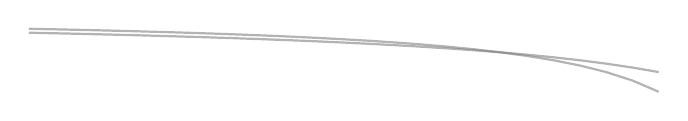
\begin{tikzpicture}[scale=1,draw opacity = 0.6]
		% abscisa y ordenada
		\tkzInit[xmax= 1,xmin=-12,ymax=1,ymin=-2]
		\tiny\tkzLabelXY[opacity=0.6,step=1, orig=false]
		% etiqueta x, f(x)
		\tkzDrawX[opacity=0.6,label=x,right=0.3]
		\tkzDrawY[opacity=0.6,label=f(x),below = -0.6]
		%dominio y función
		\draw [domain=-11:-3,thick,gray] plot(\x,{3/(\x-1)});
		\draw [domain=-11:-3,thick,gray] plot(\x,{2/(\x+1)});
	    \end{tikzpicture}
	\end{center}
	\vspace{.5cm}

	%----------b.
	\item Confirme algebraicamente los hallazgos del inicio $a)$.\\\\
	    Respuesta.-\; Sea $\dfrac{3}{x-1}<\dfrac{2}{x+1} \quad \Rightarrow \quad x<-5$\\\\

    \end{enumerate}

    %-------------------69.
    \item Para que una curva sea simétrica con respecto al eje $x$, el punto $(x, y)$ debe estar en la curva si y sólo si el punto $(x, -y)$ está en la curva. Explique por qué una curva que es simétrica con respecto al eje $x$ no es la gráfica de una función a menos que la función sea $y = 0$.\\\\
	Respuesta.-\; Esto se debe a que contradice a la definición de función. Es decir, a cada elemento $x$ se asigna un solo o único elemento $f(x)$. Si $y=0$ entonces $(x,y)=(x,-y)$ y por lo tanto se cumple la definición de función\\\\

    %--------------------70.
    \item Trescientos libros se venden en $\$ 40$ cada uno, lo que da por resultado un ingreso de $300\cdot \$ 40 $ = $\$12,000$. Por cada aumento de $\$ 5$ en el precio, se venden $25$ libros menos. Exprese el ingreso $R$ como una función del número $x$ de incrementos de $\$5$.\\\\
	Respuesta.-\; Veamos algunos ejemplos particulares:
	\begin{center}
	    \begin{tabular}{rcl}
		$300\cdot 40$&$=$&$12000$\\
		$(300 - 25)(40 + 5)$&$=$&$12375$\\
		$(300 - 50)(40 + 10)$&$=$&$12500$\\
		$(300 - 75)(40 + 15)$&$=$&$12375$\\
		$(300 - 100)(40 + 20)$&$=$&$12000$\\
	    \end{tabular}
	\end{center}
	Por lo tanto $R(x)=(300-5x)(40+x)=-125x^2 + 500x + 12000$\\\\

    %--------------------71.
    \item Se va a construir un corral con la forma de un triángulo rectángulo isósceles con catetos de longitud de $x$ pies (ft) e hipotenusa de longitud $h$ ft. Si los costos de la cerca son de $\$ 5 / ft$ para los catetos y $\$ lO/ft$ para la hipotenusa, escriba el costo total $C$ de la construcción como una función de $h$.\\\\
	Respuesta.-\; Sea $c^2+c^2=h^2 \quad \Rightarrow \quad h=c \sqrt{2} \quad \Rightarrow \quad c=h \sqrt{2}$, luego $C=2\cdot c \cdot 5 + h \cdot 10$ por lo tanto $C=10\cdot h \dfrac{1}{\sqrt{2}} + 1$\\\\

    %--------------------72.
    \item Costos industriales: Una central eléctrica se encuentra cerca de un río, donde éste tiene un ancho de 800 ft. Tender un cable de la planta a un lugar en la ciudad, 2 millas (mi) río abajo en el lado opuesto, tiene un costo de $180 por ft que cruce el río y $100 por ft en tierra a lo largo de la orilla del río.
    \begin{enumerate}[\bfseries a.]

	%----------a.
	\item Suponga que el cable va de la planta al punto $Q$, en el lado opuesto, lugar que se encuentra a $x$ ft del punto $P$, directamente opuesto a la planta. Escriba una función $C(x)$ que indique el costo de tender el cable en términos de la distancia $x$.\\\\
	    Respuesta.-\; Por el teorema de Pitágoras podemos establecer la función $C(x)$ como sigue: $$C(x)=\sqrt{x^2 + 800^2} \cdot 180 + (10560-x)\cdot 100$$

	%----------b.
	\item Genere una tabla de valores para determinar si la ubicación más barata para el punto $Q$ es menor a $2000$ ft o mayor a $2000$ ft del punto $P$.\\\\
	    Respuesta.-\;
	    \begin{center}
		\begin{tabular}{rclcl}
		    $C(x)$&$=$&$\sqrt{1900^2+800^2} + (10560-1900)\cdot 100$&$=$&$1270599.7$\\
		    $C(x)$&$=$&$\sqrt{2100^2+800^2} + (10560-2100)\cdot 100$&$=$&$1217079.5$\\\\
		\end{tabular}
	    \end{center}
	    Por lo tanto es mas barato ubicar el punto $Q$ a una distancia mayor a $2000$ ft.\\\\

    \end{enumerate}

\end{enumerate}

\section{Ejercicios}

En los ejercicios 1 y 2, determine dominios y rangos de $f,g,f+g \; y \; f\cdot g$\\\\
\begin{enumerate}[\Large \bfseries 1.]

%--------------------1.
\item $f(x)=x, \; g(x)=\sqrt{x-1}$\\\\
    Respuesta.-\; 
    \begin{center}
	\begin{tabular}{r l l}
	    Función&Dominio&Rango\\ 
	    \hline 
	    $f$ & $\forall x \in \mathbb{R}$ & $\forall f(x) \in \mathbb{R}$\\
	    $g$ & $x\geq 1$ & $f(x) \geq 0$\\
	    $f+g$ & $x\geq 1$ & $f(x)\geq 1$\\
	    $f\cdot g$ & $x\geq 1$ & $f(x) \geq 0$\\\\
	\end{tabular}
    \end{center}

%--------------------2.
\item $f(x)=\sqrt{x+1}, \; g(x)=\sqrt{x-1}$\\\\
    Respuesta.-\;
    \begin{center}
	\begin{tabular}{r l l}
	    Función&Dominio&Rango\\ 
	    \hline
	    $f$ & $x\geq -1$ & $f(x) \geq 0$\\
	    $g$ & $x\geq 1$ & $f(x) \geq 0$\\
	    $f+g$ & $x \geq 1$ & $f(x) \geq \sqrt{2}$\\
	    $f\cdot g$ & $x\geq 1$ & $f(x)\geq 0$\\\\
	\end{tabular}
    \end{center}

En los ejercicios 3 y 4, determine dominios y rangos de $f,g,f/g,g/f$.\\\\

%--------------------3.
\item $f(x)=2, \quad g(x)=x^2+1$\\\\
    Respuesta.-\; 
    \begin{center}
	\begin{tabular}{r l l}
	    Función&Dominio&Rango\\ 
	    \hline
	    $f$&$\forall\; x \in \mathbb{R}$&$f(x)=2$\\
	    $g$&$\forall \; x \in \mathbb{R}$&$f(x)\geq 1$\\
	    $f/g$&$\forall \; x \in \mathbb{R}$&$0<f(x)\leq 2$\\
	    $g/f$&$\forall \; x \in \mathbb{R}$&$f(x) \geq 0.5$\\\\
	\end{tabular}
    \end{center}

%--------------------4.
\item $f(x)=1, \quad g(x)=1 + \sqrt{x}$.\\\\
    Respuesta.-\;
    \begin{center}
	\begin{tabular}{r l l}
	    Función&Dominio&Rango\\ 
	    \hline
	    $f$&$\forall \; x \in \mathbb{R}$&$f(x)=1$\\
	    $g$&$x\geq 0$&$f(x)\geq 1$\\
	    $f/g$&$x\geq 0$&$0<f(x)\leq 1$\\
	    $g/f$&$x \geq 0$&$f(x)\geq 1$\\\\
	\end{tabular}
    \end{center}

Composición de funciones.\\\\

%--------------------5.
\item Si $f(x)=x+5$ y $g(x)=x^2-3,$ determine lo siguiente:\\\\
\begin{enumerate}[\bfseries a.]
    
    %----------a.
    \item $f(g(0)) = f(-3) = -3 + 5 = 2$\\\\

    %----------b.
    \item $g(f(0)) = g(5) = 5^2 - 3 = 22$\\\\

    %----------c.
    \item $f(g(x)) = f(x^2 - 3) = x^2 - 3 + 5 = x^2 + 2 \quad$ para $\quad D_{f\circ g} = \lbrace x \in D_g \; / \; g(x) \in D_f  \rbrace$\\\\

    %----------d.
    \item $g(f(x)) = g(x+5) = (x+5)^2 - 3 = x^2 + 10x + 25 - 3 = x^2 + 10x + 22 \quad$ para $\quad D_{g\circ f} = \lbrace x\in D_f / f(x) \in D_g \rbrace$\\\\

    %----------e.
    \item $f(f(-5)) = f(0) = 5$\\\\

    %----------f.
    \item $g(g(2)) = g(1) = 1 - 3 = -2$\\\\

    %----------g.
    \item $f(f(x)) = f(x+5) = x+ 5 + 5 = x + 10$\\\\

    %----------h.
    \item $g(g(x)) = g(x^2-3) = (x^2 - 3)^2 - 3 = x^4 - 6x^2 + 9 - 3 = x^4 - 6x^2 + 6$\\\\

\end{enumerate}

%--------------------6.
\item Si $f(x)=x-1$ y $g(x)=1/(x+1)$, determine lo siguiente.
\begin{enumerate}[\bfseries a.]
    
    %----------a.
    \item $f(g(1/2))= f(2/3) = \dfrac{2}{3} - 1 = -\dfrac{1}{3}$\\\\
    
    %----------b.
    \item $g(f(0)) = g(-1) = \dfrac{1}{-1+1} = indeterminado$\\\\
    
    %----------c.
    \item $f(g(x)) = f\left(\dfrac{1}{x+1}\right) = \dfrac{1}{x+1} - 1 = \dfrac{-x+2}{x+1} \quad $ para $\quad D_{f\circ g} = \lbrace \forall x \in D_g / g(x) \in D_f\rbrace$ \\\\
    
    %----------d.
    \item $g(f(x)) = g(x-1) = \dfrac{1}{x -1 + 1} = \dfrac{1}{x} \quad $ para $\quad D_{g\circ f} = \lbrace \forall\; x \in D_f / f(x) \in D_g \rbrace$\\\\
    
    %----------e.
    \item $f(f(-5)) = f(-6) = -6 - 1 = -7$\\\\
    
    %----------f.
    \item $g(g(2)) = g\left(\dfrac{1}{3}\right) = \dfrac{1}{\dfrac{1}{3} + 1} = \dfrac{3}{4}$\\\\
    
    %----------g.
    \item $f(f(x)) = f(x-1) = x - 2$\\\\
    
    %----------h.
    \item $g(g(x)) = g\left(\dfrac{1}{x+1}\right) = \dfrac{1}{\dfrac{1}{x+1} + 1} = \dfrac{x+1}{x+2} \quad x\neq -1, -2$\\\\

\end{enumerate}

En los ejercicios $7$ a $10$, escriba una fórmula para $f\circ g \circ h$\\\\

%--------------------7.
\item $f(x)=x+1, \quad g(x)=3x, \quad h(x)=4-x$\\\\
    Respuesta.-\; Se tiene $f(g(h(x))) = f(g(4-x)) = f(12-3x) = 12-3x + 1 = 13 - 3x \quad $ para $\quad D_{f\circ g\circ h} = \lbrace \forall \; x \in D_h / h(x) \in D_g \land g(h(x)) \in D_f\rbrace$\\\\

%--------------------8.
\item $f(x)=3x+4, \quad g(x)=2x-1, \quad h(x)=x^2$\\\\
    Respuesta.-\; Se tiene $f(g(h(x))) = f(g(x^2)) = f(2x^2-1) = 3(2x^2-1) + 4 = 6x^2 +1 $ para $D_{f\circ g\circ h}= \lbrace \forall x \in D_h / h(x) \in D_g \land g(h(x)) \in D_f \rbrace$\\\\

%--------------------9.
\item $f(x)=\sqrt{x+1},\quad \dfrac{1}{x+4}, \quad h(x)=\dfrac{1}{x}$\\\\ 
    Respuesta.-\; $f(g(h(x))) = f\left(g \left(\dfrac{1}{x}\right) \right) = f\left(\dfrac{1}{\dfrac{1}{x} + 4}\right) = \sqrt{\dfrac{1}{\dfrac{1}{x} + 4} + 1} = \sqrt{\dfrac{5x+1}{4x+1}}$ para $ x \neq 0, -\dfrac{1}{4}$.\\\\

%--------------------10.
\item $f(x)=\dfrac{x+2}{3-x}, \quad g(x)=\dfrac{x^2}{x^2+1}, \quad h(x)=\sqrt{2-x}$\\\\
    Respuesta.-\; $f\left( g \left( \sqrt{2-x}\right)\right) = f\left( \dfrac{|2-x|}{|2-x|+1}\right) = \dfrac{\dfrac{|2-x|}{|2-x|+1} + 2}{3 - \left(\dfrac{|2-x|}{|2-x|+1}\right)}$\\\\

Sean $f(x)=x-3, \quad g(x)=\sqrt{x}, \quad h(x)=x^3$ y $j(x)=2x$. Exprese cada una de las funciones de los ejercicios $11$ y $12$ como una composición de funciones que incluyan a una o más de $f,g,h$ y $j$.\\\\

%--------------------11.
\item
\begin{enumerate}[\bfseries a.]
    
    %----------a.
    \item $y=\sqrt{x}-3 \Rightarrow f(\sqrt{x}) \Rightarrow f(g(x))$\\\\

    %----------b.
    \item $y=2\sqrt{x} \Rightarrow j(\sqrt{x}) \Rightarrow j(g(x))$\\\\

    %----------c.
    \item $y=x^{1/4} \Rightarrow g(\sqrt{x}) \Rightarrow g(g(x))$\\\\

    %----------d.
    \item $y=4x \Rightarrow j(j(x))$\\\\

    %----------e.
    \item $y=\sqrt{(x-3)^3} \Rightarrow g((x-3)^3) \Rightarrow g(h(x-3)) \Rightarrow g(h(f(x)))$\\\\

    %----------f.
    \item $y=(2x-6)^3 \Rightarrow h(2x-6) = h(j(x-3)) = h(j(f(x))$.\\\\ 

\end{enumerate}

%--------------------12.
\item 
\begin{enumerate}[\bfseries a.]
    
    %----------a.
    \item $y=2x-3 \Rightarrow f(2x) \Rightarrow f(j(x))$\\\\
    
    %----------b.
    \item $y=x^{3/2} \Rightarrow g(x^3) \Rightarrow g(h(x))$\\\\
    
    %----------c.
    \item $y=x^9 \Rightarrow h(x^3) \Rightarrow h(h(x))$\\\\
    
    %----------d.
    \item $y=x-6 \Rightarrow f(f(x))$\\\\
    
    %----------e.
    \item $y=2\sqrt{x-3} \Rightarrow j(\sqrt{x-3}) \Rightarrow j(g(x-3)) \Rightarrow j(g(f(x)))$\\\\
    
    %----------f.
    \item $y=\sqrt{x^3-3} \Rightarrow g(x^3-3) \Rightarrow g(f(x^3)) \Rightarrow g(f(h(x)))$\\\\
    
\end{enumerate}

%--------------------13.
\item Copie complete la siguiente tabla:\\
\begin{center}
    \begin{tabular}{c c c c}
	     & $g(x)$ & $f(x)$ & $(f\circ g)(x)$\\\\
	\hline \\
	$a.$ & $x-7$ & $\sqrt{x}$ & $\sqrt{x-7}$\\\\
	$b.$ & $x+2$ & $2x$ & $3x+6$\\\\
	$c.$ & $x^2$ & $\sqrt{x-5}$ & $\sqrt{x^2-5}$\\\\
	$d.$ & $\dfrac{x}{x-1}$ & $\sqrt{x}{x-1}$ & $\dfrac{x}{(x-1)^2}$\\\\
	$e.$ & $x^3$ & $1+\dfrac{1}{x}$ & $1+\dfrac{1}{x^3}$\\\\
	$f.$ & $\dfrac{1}{x}$ & $\sqrt{x}$ & $\sqrt{\dfrac{1}{x}}$\\\\
    \end{tabular}
\end{center}

%--------------------14.
\item  Copie y complete la siguiente tabla.
\begin{center}
    \begin{tabular}{cccc}
	&$g(x)$&$f(x)$&$(f\circ g)(x)$\\\\
	\hline\\
	$a.$&$\dfrac{1}{x-1}$&$|x|$&$\left| \dfrac{1}{x-1}\right|$\\\\
	$b.$&$x+2$&$\dfrac{x-1}{x}$&$\dfrac{x}{x+1}$\\\\
	$c.$&$x^2$&$\sqrt{x}$&$|x|$\\\\
	$d.$&$\sqrt{x}$&$x^2$&$|x|$\\\\
    \end{tabular}
\end{center}

%--------------------15.
\item Evalúe cada expresión utilizando la siguiente tabla de valores.\\\\
\begin{enumerate}[\bfseries a.]

    %----------a.
    \item $f(g(-1)) = f(0) = -2$\\\\

    %----------b.
    \item $g(f(0)) = g(-2) = 2$\\\\ 

    %----------c.
    \item $f(f(-1)) = f(0) = -2$\\\\

    %----------d.
    \item $g(g(2)) = g(0) = 0$\\\\

    %----------e.
    \item $g(f(-2)) = g(1) = -1$\\\\

    %----------f.
    \item $f(g(1)) = f(-1) = 0$\\\\

\end{enumerate}

%--------------------16.
\item Evalúe cada expresión con el uso de las funciones.
$$f(x) = 2-x, \qquad g(x) = \left\{\begin{array}{lr} -x,& -2\leq x < 0\\ \\x-1, & 0\leq x \leq 2\\ \end{array}\right.$$\\
\begin{enumerate}[\bfseries a.]
    
    %----------a.
    \item $f(g(0)) = f(0-1) = 2 + 1 = 3$\\\\
    
    %----------b.
    \item $g(f(0)) = g(2) = 1$\\\\
    
    %----------c.
    \item $g(g(-1)) = g(1) = 0$\\\\
    
    %----------d.
    \item $f(f(2)) = f(0) = 2$\\\\
    
    %----------e.
    \item $g(f(0)) = g(2) = 1$\\\\
    
    %----------f.
    \item $f(g(1/2)) = f(-1/2) = 5/2$\\\\
\end{enumerate}

En los ejercicios 17 y 18, (a) escriba fórmulas para $f\circ g$ y $g\circ f$, luego determine (b) el dominio y (c) el rango de cada una.\\\\

%--------------------17.
\item $f(x) =\sqrt{x+1}, \quad g(x)=\dfrac{1}{x}$\\\\
    Respuesta.-\; 
    Para $f\circ g = f(g(x)) = f\left(\dfrac{1}{x}\right) = \sqrt{\dfrac{1}{x}+1}$ de donde el dominio viene dado por $x>0 \; \land \; x\leq -1$, y el rango viene dado por $f(x)\geq 0$. Luego para $g\circ f = g(f(x)) = g(\sqrt{x+1}) = \dfrac{1}{\sqrt{x+1}}$ de donde el dominio es $x>-1$ y el rango $\forall \; \mathbb{R}, x\neq 0$.\\\\ 

%--------------------18.
\item $f(x) = x^2, \quad g(x) = 1 - \sqrt{x}$\\\\
    Respuesta.-\; Para $f(1-\sqrt{x}) = (1-\sqrt{x})^2 = 1 - 2 \sqrt{x} + |x|$ el dominio viene dado por $x\geq 0$ y el rango por $f(g(x)) \geq 0$.\\
    Luego para $g(x^2) = 1 - \sqrt{x^2} = 1 - |x|$ el dominio viene dado por $x\geq 0$ y el rango $g(f(x)) \geq 1$.\\\\

%-------------------19.
\item Sea $f(x) = \dfrac{x}{x-2}$. Determine una función $y=g(x)$ de modo que $(f\circ g)(x) = x$.\\\\
    Respuesta.-\; Sea $f(g(x))=x$ entonces $\dfrac{g(x)}{g(x)-2} = x$ ó $\dfrac{y}{y-2}=x$ por lo tanto $y=g(x)=\dfrac{-2x}{1-x}$.\\\\ 

%--------------------20.
\item Sea $f(x)=2x^3 - 4$. Determine una función $y=g(x)$ de modo que $(f\circ g)(x)=x+2$.\\\\
    Respuesta.-\; Similar al anterior ejercicio tenemos que $2y^3 - 4 = x+2$ de donde nos queda $$y=g(x)=\sqrt[3]{\dfrac{x+6}{2}}$$\\

Traslación de gráficas.\\\\

%--------------------21.
\item La siguiente figura muestra la gráfica de $y=-x^2$ desplazada a dos posiciones nuevas. Escriba las ecuaciones de las gráficas nuevas.\\\\
    Respuesta.-\; 
    \begin{enumerate}[a)]
	\item $y=-(x+7)^2$\\
	\item $y=-(x-4)^2$\\\\
    \end{enumerate}

%-------------------22.
\item La siguiente figura muestra la gráfica de $y=x^2$ desplazada a dos posiciones nuevas. Escriba las ecuaciones de las gráficas nuevas.\\\\
    Respuesta.-\; 
    \begin{enumerate}[a)]
	\item $y=x^2 + 3$\\
	\item $x^2 - 5$\\\\
    \end{enumerate}

%--------------------23.
\item Relacione las ecuaciones listadas en los incisos $a)$ a $d)$ con las gráficas de la figura.\\\\
    Respuesta.-\;
    \begin{enumerate}[\bfseries a)]

	%----------a)
	\item $y=(x-1)^2 - 4 = $ Posición 4.\\\\

	%----------b)
	\item $y=(x-2)^2 + 2 = $ Posición 1.\\\\

	%----------c)
	\item $y=(x+2)^2 + 2 = $ Posición 2.\\\\

	%----------d)
	\item $y=(x+3)^2 - 2 = $ Posición 3.\\\\
    \end{enumerate}

%--------------------24.
\item La siguiente figura muestra la gráfica de $y=-x^2$ desplazada a cuatro posiciones nuevas. Escriba una ecuación para cada nueva gráfica.\\\\
    Respuesta.-\; 
    \begin{enumerate}[a)]
	\item $y=-(x-1)^2 + 4$\\
	\item $y=-(x+2)^2 + 3$\\
	\item $y=-(x+4)^2 - 1$\\
	\item $y=-(x-2)^2$\\\\
    \end{enumerate}

En los ejercicios $25$ a $34$ se establece cuántas unidades y en qué direcciones se trasladarán las gráficas de las ecuaciones dadas. Proporcione una ecuación para la gráfica desplazada: después, en el mismo plano cartesiano, trace la gráfica de la función original y la gráfica de la ecuación desplazada, anotando junto a cada gráfica la ecuación que le corresponda.\\\\

%--------------------25.
\item $x^2+y^2 = 49$ abajo $3$, izquierda $2$.\\\\ 
    Respuesta.-\; $$y=\sqrt{49-(x+2)^2} - 3 \quad \Rightarrow \quad (x+2)^2 + (y+3)^2 = 49$$
	\begin{center}
	    \begin{tikzpicture}[scale=.6, draw opacity = 0.6]
		% abscisa y ordenada
		\tkzInit[xmax= 7,xmin=-7,ymax=7,ymin=-1]
		\tiny\tkzLabelXY[opacity=0.6,step=1, orig=false]
		% etiqueta x, f(x)
		\tkzDrawX[opacity=0.6,label=x,right=0.3]
		\tkzDrawY[opacity=0.6,label=f(x),below = -0.6]
		%dominio y función
		\draw [domain=-8:4,thick,gray] plot(\x,{(49-(\x+2)^2)^(1/2) - 3});
		\draw [domain=-6:6,thick,gray] plot(\x,{(49-\x*\x)^(1/2)});
	    \end{tikzpicture}
	\end{center}
	\vspace{.5cm}

%--------------------26.
\item $x^2 + y^2 = 25$ Arriba $3$, izquierda $4$\\\\
    Respuesta.-\; $$(x+4)^2 + (y-3)^2 = 25$$
	\begin{center}
	    \begin{tikzpicture}[scale=.6, draw opacity = 0.6]
		% abscisa y ordenada
		\tkzInit[xmax= 5,xmin=-8,ymax=8,ymin=-1]
		\tiny\tkzLabelXY[opacity=0.6,step=1, orig=false]
		% etiqueta x, f(x)
		\tkzDrawX[opacity=0.6,label=x,right=0.3]
		\tkzDrawY[opacity=0.6,label=f(x),below = -0.6]
		%dominio y función
		\draw [domain=-8:0,thick,gray] plot(\x,{(25-(\x+4)^2)^(1/2) + 3});
		\draw [domain=-4:4,thick,gray] plot(\x,{(25-\x*\x)^(1/2)});
	    \end{tikzpicture}
	\end{center}
	\vspace{.5cm}

%--------------------27.
\item $y=x^3$ Izquierda $1$, abajo $1$.\\\\
    Respuesta.-\; $$y=(x+1)^3 - 1$$
	\begin{center}
	    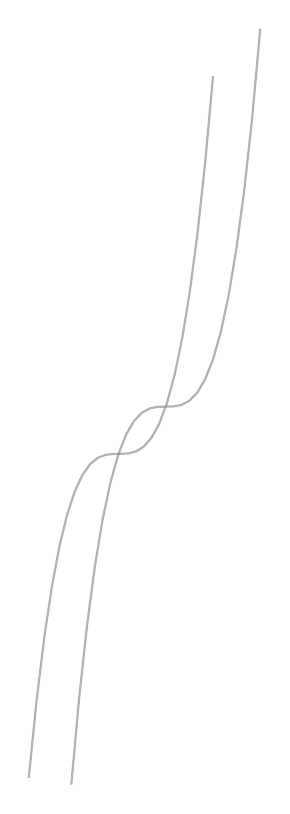
\begin{tikzpicture}[scale=.6, draw opacity = 0.6]
		% abscisa y ordenada
		\tkzInit[xmax= 3,xmin=-3,ymax=8,ymin=-8]
		\tiny\tkzLabelXY[opacity=0.6,step=1, orig=false]
		% etiqueta x, f(x)
		\tkzDrawX[opacity=0.6,label=x,right=0.3]
		\tkzDrawY[opacity=0.6,label=f(x),below = -0.6]
		%dominio y función
		\draw [domain=-2:2,thick,gray] plot(\x,{\x^3});
		\draw [domain=-2.9:1,thick,gray] plot(\x,{(\x+1)^3 - 1});
	    \end{tikzpicture}
	\end{center}
	\vspace{.5cm}

%--------------------28.
\item $y = x^{2/3}$ Derecha 1, abajo 1\\\\
    Respuesta.-\; $$y=(x-1)^{2/3}  - 1$$
	\begin{center}
	    \begin{tikzpicture}[scale=.6, draw opacity = 0.6]
		% abscisa y ordenada
		\tkzInit[xmax= 5,xmin=-3,ymax=2,ymin=-2]
		\tiny\tkzLabelXY[opacity=0.6,step=1, orig=false]
		% etiqueta x, f(x)
		\tkzDrawX[opacity=0.6,label=x,right=0.3]
		\tkzDrawY[opacity=0.6,label=f(x),below = -0.6]
		%dominio y función
		\draw [domain=-2:2,thick,gray] plot(\x,{\x^(2/3)});
		\draw [domain=1:4,thick,gray] plot(\x,{(\x-1)^(2/3) - 1});
	    \end{tikzpicture}
	\end{center}
	\vspace{.5cm}

%--------------------29
\item $y = \sqrt{x}$ Izquierda 0.81\\\\
    Respuesta.-\; $$\sqrt{x+0.81}$$
	\begin{center}
	    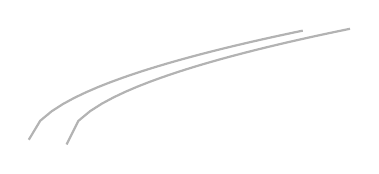
\begin{tikzpicture}[scale=.6, draw opacity = 0.6]
		% abscisa y ordenada
		\tkzInit[xmax= 6,xmin=-2,ymax=2,ymin=-1]
		\tiny\tkzLabelXY[opacity=0.6,step=1, orig=false]
		% etiqueta x, f(x)
		\tkzDrawX[opacity=0.6,label=x,right=0.3]
		\tkzDrawY[opacity=0.6,label=f(x),below = -0.6]
		%dominio y función
		\draw [domain=0:6, thick,gray] plot(\x,{\x^(1/2)});
		\draw [domain=-.8:5,thick,gray] plot(\x,{(\x+0.81)^(1/2)});
	    \end{tikzpicture}
	\end{center}
	\vspace{.5cm}

%--------------------30.
\item $y = - \sqrt{x}$ Derecha 3 \\\\ 
    Respuesta.-\; $$y=-\sqrt{x-3}$$
	\begin{center}
	    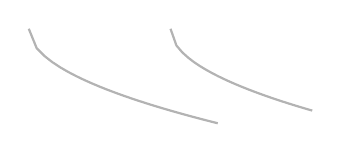
\begin{tikzpicture}[scale=.6, draw opacity = 0.6]
		% abscisa y ordenada
		\tkzInit[xmax= 7,xmin=-1,ymax=1,ymin=-3]
		\tiny\tkzLabelXY[opacity=0.6,step=1, orig=false]
		% etiqueta x, f(x)
		\tkzDrawX[opacity=0.6,label=x,right=0.3]
		\tkzDrawY[opacity=0.6,label=f(x),below = -0.6]
		%dominio y función
		\draw [domain=0:4,thick,gray] plot(\x,{-1*(\x)^(1/2)});
		\draw [domain=3:6,thick,gray] plot(\x,{-1*(\x-3)^(1/2)});
	    \end{tikzpicture}
	\end{center}
	\vspace{.5cm}

%--------------------31.
\item  $y = 2x - 7$ Arriba 7 \\\\ 
    Respuesta.-\; $$y=2x$$
	\begin{center}
	    \begin{tikzpicture}[scale=.6, draw opacity = 0.6]
		% abscisa y ordenada
		\tkzInit[xmax= 4,xmin=-3,ymax=6,ymin=-9]
		\tiny\tkzLabelXY[opacity=0.6,step=1, orig=false]
		% etiqueta x, f(x)
		\tkzDrawX[opacity=0.6,label=x,right=0.3]
		\tkzDrawY[opacity=0.6,label=f(x),below = -0.6]
		%dominio y función
		\draw [domain=-1:3,thick,gray] plot(\x,{2*\x - 7});
		\draw [domain=-1:3,thick,gray] plot(\x,{2*\x});
	    \end{tikzpicture}
	\end{center}
	\vspace{.5cm}

%--------------------32.
\item $y = \dfrac{1}{2} (x + 1) + 5$ Abajo 5, derecha 1 \\\\ 
    Respuesta.-\; $$y=\dfrac{1}{2}x$$
	\begin{center}
	    \begin{tikzpicture}[scale=.6, draw opacity = 0.6]
		% abscisa y ordenada
		\tkzInit[xmax= 5,xmin=-6,ymax=7,ymin=-2]
		\tiny\tkzLabelXY[opacity=0.6,step=1, orig=false]
		% etiqueta x, f(x)
		\tkzDrawX[opacity=0.6,label=x,right=0.3]
		\tkzDrawY[opacity=0.6,label=f(x),below = -0.6]
		%dominio y función
		\draw [domain=-5:3,thick,gray] plot(\x,{(1/2)*(\x + 1) + 5});
		\draw [domain=-4:4,thick,gray] plot(\x,{(1/2)*\x});
	    \end{tikzpicture}
	\end{center}
	\vspace{.5cm}

%--------------------33.
\item $y=\dfrac{1}{x}$ Arriba 1, derecha 1\\\\ 
    Respuesta.-\; $$y=\dfrac{1}{x-1}  + 1$$
	\begin{center}
	    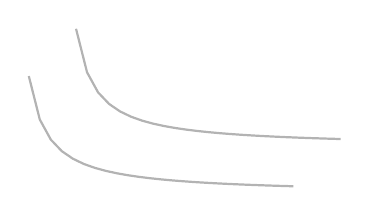
\begin{tikzpicture}[scale=.6, draw opacity = 0.6]
		% abscisa y ordenada
		\tkzInit[xmax= 7,xmin=-1,ymax=4,ymin=-1]
		\tiny\tkzLabelXY[opacity=0.6,step=1, orig=false]
		% etiqueta x, f(x)
		\tkzDrawX[opacity=0.6,label=x,right=0.3]
		\tkzDrawY[opacity=0.6,label=f(x),below = -0.6]
		%dominio y función
		\draw [domain=.4:6,thick,gray] plot(\x,{1/\x});
		\draw [domain=1.4:7,thick,gray] plot(\x,{1/(\x-1) + 1});
	    \end{tikzpicture}
	\end{center}
	\vspace{.5cm}

%--------------------34.
\item $y=\dfrac{1}{x^2}$ Izquierda 2, abajo 1 \\\\ 
    Respuesta.-\; $$y=\dfrac{1}{(x+2)^2} - 1$$
	\begin{center}
	    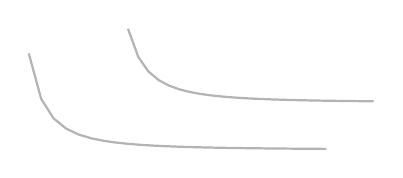
\begin{tikzpicture}[scale=.6, draw opacity = 0.6]
		% abscisa y ordenada
		\tkzInit[xmax= 8,xmin=-2,ymax=2,ymin=-1]
		\tiny\tkzLabelXY[opacity=0.6,step=1, orig=false]
		% etiqueta x, f(x)
		\tkzDrawX[opacity=0.6,label=x,right=0.3]
		\tkzDrawY[opacity=0.6,label=f(x),below = -0.6]
		%dominio y función
		\draw [domain=.8:6,thick,gray] plot(\x,{1/\x^2});
		\draw [domain=-1.3:5,thick,gray] plot(\x,{(1/(\x+2)^2) - 1});
	    \end{tikzpicture}
	\end{center}
	\vspace{.5cm}

Grafique las funciones de los ejercicios $35$ a $54$\\\\

%--------------------35.
\item $y=\sqrt{x+4}$\\\\
    Respuesta.-\;
	\begin{center}
	    \begin{tikzpicture}[scale=.6, draw opacity = 0.6]
		% abscisa y ordenada
		\tkzInit[xmax= 5,xmin=-4,ymax=3,ymin=-1]
		\tiny\tkzLabelXY[opacity=0.6,step=1, orig=false]
		% etiqueta x, f(x)
		\tkzDrawX[opacity=0.6,label=x,right=0.3]
		\tkzDrawY[opacity=0.6,label=f(x),below = -0.6]
		%dominio y función
		\draw [domain=-4:4,thick,gray] plot(\x,{(\x+4)^(1/2)});
	    \end{tikzpicture}
	\end{center}
	\vspace{.5cm}

%--------------------36.
\item $y=\sqrt{9-x}$\\\\
    Respuesta.-\;
	\begin{center}
	    \begin{tikzpicture}[scale=.6, draw opacity = 0.6]
		% abscisa y ordenada
		\tkzInit[xmax= 9,xmin=-8,ymax=4,ymin=-1]
		\tiny\tkzLabelXY[opacity=0.6,step=1, orig=false]
		% etiqueta x, f(x)
		\tkzDrawX[opacity=0.6,label=x,right=0.3]
		\tkzDrawY[opacity=0.6,label=f(x),below = -0.6]
		%dominio y función
		\draw [domain=-8:9,thick,gray] plot(\x,{(9-\x)^(1/2)});
	    \end{tikzpicture}
	\end{center}
	\vspace{.5cm}

%--------------------37.
\item $y=|x-2|$\\\\
    Respuesta.-\;
	\begin{center}
	    \begin{tikzpicture}[scale=.6, draw opacity = 0.6]
		% abscisa y ordenada
		\tkzInit[xmax= 6,xmin=-3,ymax=5,ymin=-1]
		\tiny\tkzLabelXY[opacity=0.6,step=1, orig=false]
		% etiqueta x, f(x)
		\tkzDrawX[opacity=0.6,label=x,right=0.3]
		\tkzDrawY[opacity=0.6,label=f(x),below = -0.6]
		%dominio y función
		\draw [domain=-2:6,thick,gray] plot(\x,{abs(\x-2)});
	    \end{tikzpicture}
	\end{center}
	\vspace{.5cm}
    
%--------------------38.
\item $y=|1-x|-1$\\\\
    Respuesta.-\;
	\begin{center}
	    \begin{tikzpicture}[scale=.6, draw opacity = 0.6]
		% abscisa y ordenada
		\tkzInit[xmax= 7,xmin=-4,ymax=5,ymin=-1]
		\tiny\tkzLabelXY[opacity=0.6,step=1, orig=false]
		% etiqueta x, f(x)
		\tkzDrawX[opacity=0.6,label=x,right=0.3]
		\tkzDrawY[opacity=0.6,label=f(x),below = -0.6]
		%dominio y función
		\draw [domain=-4:6,thick,gray] plot(\x,{abs(1-\x)-1});
	    \end{tikzpicture}
	\end{center}
	\vspace{.5cm}

%--------------------39.
\item $y=1+\sqrt{x-1}$\\\\
    Respuesta.-\;
	\begin{center}
	    \begin{tikzpicture}[scale=.6, draw opacity = 0.6]
		% abscisa y ordenada
		\tkzInit[xmax= 7,xmin=-1,ymax=3,ymin=-1]
		\tiny\tkzLabelXY[opacity=0.6,step=1, orig=false]
		% etiqueta x, f(x)
		\tkzDrawX[opacity=0.6,label=x,right=0.3]
		\tkzDrawY[opacity=0.6,label=f(x),below = -0.6]
		%dominio y función
		\draw [domain=1:6,thick,gray] plot(\x,{1 + (\x-1)^(1/2)});
	    \end{tikzpicture}
	\end{center}
	\vspace{.5cm}

%--------------------40.
    \item $y=1 - \sqrt{x}$\\\\
    Respuesta.-\;
	\begin{center}
	    \begin{tikzpicture}[scale=.6, draw opacity = 0.6]
		% abscisa y ordenada
		\tkzInit[xmax= 7,xmin=-1,ymax=1,ymin=-2]
		\tiny\tkzLabelXY[opacity=0.6,step=1, orig=false]
		% etiqueta x, f(x)
		\tkzDrawX[opacity=0.6,label=x,right=0.3]
		\tkzDrawY[opacity=0.6,label=f(x),below = -0.6]
		%dominio y función
		\draw [domain=0:6,thick,gray] plot(\x,{1-\x^(1/2)});
	    \end{tikzpicture}
	\end{center}
	\vspace{.5cm}

%--------------------41.
    \item $y=(x+1)^{2/3}$\\\\
    Respuesta.-\;
	\begin{center}
	    \begin{tikzpicture}[scale=.6, draw opacity = 0.6]
		% abscisa y ordenada
		\tkzInit[xmax=6,xmin=-2,ymax=3,ymin=-1]
		\tiny\tkzLabelXY[opacity=0.6,step=1, orig=false]
		% etiqueta x, f(x)
		\tkzDrawX[opacity=0.6,label=x,right=0.3]
		\tkzDrawY[opacity=0.6,label=f(x),below = -0.6]
		%dominio y función
		\draw [domain=-1:5,thick,gray] plot(\x,{(\x+1)^(2/3)});
	    \end{tikzpicture}
	\end{center}
	\vspace{.5cm}

%--------------------42.
    \item $y=(x-8)^{2/3}$\\\\
    Respuesta.-\;
	\begin{center}
	    \begin{tikzpicture}[scale=.6, draw opacity = 0.6]
		% abscisa y ordenada
		\tkzInit[xmax= 12,xmin=0,ymax=2,ymin=-1]
		\tiny\tkzLabelXY[opacity=0.6,step=1, orig=false]
		% etiqueta x, f(x)
		\tkzDrawX[opacity=0.6,label=x,right=0.3]
		\tkzDrawY[opacity=0.6,label=f(x),below = -0.6]
		%dominio y función
		\draw [domain=8:12,thick,gray] plot(\x,{(\x-8)^(2/3)});
	    \end{tikzpicture}
	\end{center}
	\vspace{.5cm}

%--------------------43.
\item $y=1-x^{2/3}$\\\\
    Respuesta.-\;
	\begin{center}
	    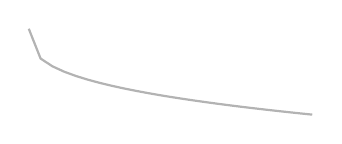
\begin{tikzpicture}[scale=.6, draw opacity = 0.6]
		% abscisa y ordenada
		\tkzInit[xmax= 7,xmin=-1,ymax=2,ymin=-1]
		\tiny\tkzLabelXY[opacity=0.6,step=1, orig=false]
		% etiqueta x, f(x)
		\tkzDrawX[opacity=0.6,label=x,right=0.3]
		\tkzDrawY[opacity=0.6,label=f(x),below = -0.6]
		%dominio y función
		\draw [domain=0:6,thick,gray] plot(\x,{1 - \x^(1/3)});
	    \end{tikzpicture}
	\end{center}
	\vspace{.5cm}

%--------------------44.
\item $y+4=x^{2/3}$\\\\
    Respuesta.-\;
	\begin{center}
	    \begin{tikzpicture}[scale=.6, draw opacity = 0.6]
		% abscisa y ordenada
		\tkzInit[xmax= 8,xmin=-2,ymax=1,ymin=-4]
		\tiny\tkzLabelXY[opacity=0.6,step=1, orig=false]
		% etiqueta x, f(x)
		\tkzDrawX[opacity=0.6,label=x,right=0.3]
		\tkzDrawY[opacity=0.6,label=f(x),below = -0.6]
		%dominio y función
		\draw [domain=0:6,thick,gray] plot(\x,{\x^(2/3) - 4});
	    \end{tikzpicture}
	\end{center}
	\vspace{.5cm}

%--------------------45.
\item $y=\sqrt[3]{x-1} - 1$\\\\
    Respuesta.-\;
	\begin{center}
	    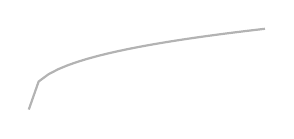
\begin{tikzpicture}[scale=.6, draw opacity = 0.6]
		% abscisa y ordenada
		\tkzInit[xmax= 8,xmin=-2,ymax=2,ymin=-1]
		\tiny\tkzLabelXY[opacity=0.6,step=1, orig=false]
		% etiqueta x, f(x)
		\tkzDrawX[opacity=0.6,label=x,right=0.3]
		\tkzDrawY[opacity=0.6,label=f(x),below = -0.6]
		%dominio y función
		\draw [domain=1:6,thick,gray] plot(\x,{(\x-1)^(1/3)-1});
	    \end{tikzpicture}
	\end{center}
	\vspace{.5cm}

%--------------------46.
\item $y=(x+2)^{3/2} + 1$\\\\
    Respuesta.-\;
	\begin{center}
	    \begin{tikzpicture}[scale=.6, draw opacity = 0.6]
		% abscisa y ordenada
		\tkzInit[xmax= 4,xmin=-3,ymax=8,ymin=-1]
		\tiny\tkzLabelXY[opacity=0.6,step=1, orig=false]
		% etiqueta x, f(x)
		\tkzDrawX[opacity=0.6,label=x,right=0.3]
		\tkzDrawY[opacity=0.6,label=f(x),below = -0.6]
		%dominio y función
		\draw [domain=-2:2,thick,gray] plot(\x,{(\x+2)^(3/2) + 1});
	    \end{tikzpicture}
	\end{center}
	\vspace{.5cm}

%--------------------47.
\item $y=\dfrac{1}{x-2}$\\\\
    Respuesta.-\;
	\begin{center}
	    \begin{tikzpicture}[scale=.6, draw opacity = 0.6]
		% abscisa y ordenada
		\tkzInit[xmax= 8,xmin=-2,ymax=13,ymin=-6]
		\tiny\tkzLabelXY[opacity=0.6,step=1, orig=false]
		% etiqueta x, f(x)
		\tkzDrawX[opacity=0.6,label=x,right=0.3]
		\tkzDrawY[opacity=0.6,label=f(x),below = -0.6]
		%dominio y función
		\draw [domain=0.1:6,thick,gray] plot(\x,{1/(\x-2)});
	    \end{tikzpicture}
	\end{center}
	\vspace{.5cm}

%--------------------48.
\item $y=\dfrac{1}{x}-2$\\\\
    Respuesta.-\;
	\begin{center}
	    \begin{tikzpicture}[scale=.6, draw opacity = 0.6]
		% abscisa y ordenada
		\tkzInit[xmax= 8,xmin=-2,ymax=7,ymin=-2]
		\tiny\tkzLabelXY[opacity=0.6,step=1, orig=false]
		% etiqueta x, f(x)
		\tkzDrawX[opacity=0.6,label=x,right=0.3]
		\tkzDrawY[opacity=0.6,label=f(x),below = -0.6]
		%dominio y función
		\draw [domain=.1:6,thick,gray] plot(\x,{1/\x - 2});
	    \end{tikzpicture}
	\end{center}
	\vspace{.5cm}

%--------------------49.
\item $y=\dfrac{1}{x}+2$\\\\
    Respuesta.-\;
	\begin{center}
	    \begin{tikzpicture}[scale=.6, draw opacity = 0.6]
		% abscisa y ordenada
		\tkzInit[xmax= 8,xmin=-2,ymax=6,ymin=-1]
		\tiny\tkzLabelXY[opacity=0.6,step=1, orig=false]
		% etiqueta x, f(x)
		\tkzDrawX[opacity=0.6,label=x,right=0.3]
		\tkzDrawY[opacity=0.6,label=f(x),below = -0.6]
		%dominio y función
		\draw [domain=.2:6,thick,gray] plot(\x,{1/\x + 2});
	    \end{tikzpicture}
	\end{center}
	\vspace{.5cm}

%--------------------50.
\item $y=\dfrac{1}{x+2}$\\\\
    Respuesta.-\;
	\begin{center}
	    \begin{tikzpicture}[scale=.6, draw opacity = 0.6]
		% abscisa y ordenada
		\tkzInit[xmax= 7,xmin=-2,ymax=2,ymin=-1]
		\tiny\tkzLabelXY[opacity=0.6,step=1, orig=false]
		% etiqueta x, f(x)
		\tkzDrawX[opacity=0.6,label=x,right=0.3]
		\tkzDrawY[opacity=0.6,label=f(x),below = -0.6]
		%dominio y función
		\draw [domain=-1.6:5,thick,gray] plot(\x,{1/(\x+2)});
	    \end{tikzpicture}
	\end{center}
	\vspace{.5cm}

%--------------------51.
\item $y=\dfrac{1}{(x-1)^2}$\\\\
    Respuesta.-\;
	\begin{center}
	    \begin{tikzpicture}[scale=.6, draw opacity = 0.6]
		% abscisa y ordenada
		\tkzInit[xmax= 8,xmin=-2,ymax=3,ymin=-1]
		\tiny\tkzLabelXY[opacity=0.6,step=1, orig=false]
		% etiqueta x, f(x)
		\tkzDrawX[opacity=0.6,label=x,right=0.3]
		\tkzDrawY[opacity=0.6,label=f(x),below = -0.6]
		%dominio y función
		\draw [domain=1.5:8,thick,gray] plot(\x,{1/(\x-1)^2});
	    \end{tikzpicture}
	\end{center}
	\vspace{.5cm}

%--------------------52.
\item $y=\dfrac{1}{x^2} - 1$\\\\
    Respuesta.-\;
	\begin{center}
	    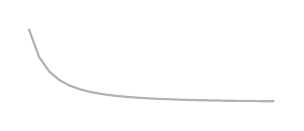
\begin{tikzpicture}[scale=.6, draw opacity = 0.6]
		% abscisa y ordenada
		\tkzInit[xmax= 8,xmin=-2,ymax=2,ymin=-1]
		\tiny\tkzLabelXY[opacity=0.6,step=1, orig=false]
		% etiqueta x, f(x)
		\tkzDrawX[opacity=0.6,label=x,right=0.3]
		\tkzDrawY[opacity=0.6,label=f(x),below = -0.6]
		%dominio y función
		\draw [domain=.8:6,thick,gray] plot(\x,{1/\x^2 - 1});
	    \end{tikzpicture}
	\end{center}
	\vspace{.5cm}

%--------------------53.
\item $y=\dfrac{1}{x^2}+1$\\\\
    Respuesta.-\;
	\begin{center}
	    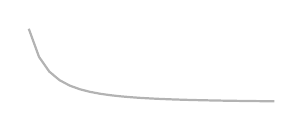
\begin{tikzpicture}[scale=.6, draw opacity = 0.6]
		% abscisa y ordenada
		\tkzInit[xmax= 8,xmin=-2,ymax=2,ymin=-1]
		\tiny\tkzLabelXY[opacity=0.6,step=1, orig=false]
		% etiqueta x, f(x)
		\tkzDrawX[opacity=0.6,label=x,right=0.3]
		\tkzDrawY[opacity=0.6,label=f(x),below = -0.6]
		%dominio y función
		\draw [domain=.8:6,thick,gray] plot(\x,{1/\x^2 + 1});
	    \end{tikzpicture}
	\end{center}
	\vspace{.5cm}

%--------------------54.
\item $y=\dfrac{1}{(x+1)^2}$\\\\
    Respuesta.-\;
	\begin{center}
	    
\begin{tikzpicture}[scale=.6, draw opacity = 0.6]
		% abscisa y ordenada
		\tkzInit[xmax= 8,xmin=-2,ymax=2,ymin=-1]
		\tiny\tkzLabelXY[opacity=0.6,step=1, orig=false]
		% etiqueta x, f(x)
		\tkzDrawX[opacity=0.6,label=x,right=0.3]
		\tkzDrawY[opacity=0.6,label=f(x),below = -0.6]
		%dominio y función
		\draw [domain=.1:7,thick,gray] plot(\x,{1/(\x+1)^2});
	    \end{tikzpicture}
	\end{center}
	\vspace{.5cm}

%--------------------55.
\item La siguiente figura muestra la gráfica de una función $f(x)$ con dominio $[0, 2]$ y rango $[0, 1]$. Determine los dominios y los rangos de las siguientes funciones, y trace sus gráficas.
    \begin{enumerate}[\bfseries a)]

	%----------a)
	\item $f(x)+2$\\\\
	    Respuesta.-\; El dominio viene dado por $[0,2]$ y el rango por $[2,3]$\\\\

	%----------b)
	\item $f(x)-1$\\\\
	    Respuesta.-\; El dominio es $[0,2]$ y el rango $[-1,0]$.\\\\ 

	%----------c)
	\item $2f(x)$\\\\
	    Respuesta.-\; El dominio es $[0,2]$ y el rango $[0,2]$.\\\\ 

	%----------d)
	\item $-f(x)$\\\\
	    Respuesta.-\; El dominio es $[0,2]$ y el rango $[-1,0]$.\\\\ 

	%----------e)
	\item $f(x+2)$\\\\
	    Respuesta.-\; El dominio es $[-2,0]$ y el rango $[0,1]$.\\\\ 

	%----------f)
	\item $f(x-1)$\\\\
	    Respuesta.-\; El dominio es $[1,3]$ y el rango $[0,1]$.\\\\ 

	%----------g)
	\item $f(-x)$\\\\
	    Respuesta.-\; El dominio es $[-2,0]$ y el rango $[0,1]$.\\\\ 

	%----------h)
	\item $-f(x+1)+1$\\\\
	    Respuesta.-\; El dominio es $[-1,1]$ y el rango $[0,1]$.\\\\ 

    \end{enumerate}

%--------------------56.
\item La siguiente figura muestra la gráfica de una función $g(t)$ con dominio $[-4, 0]$ y rango $[-3, 0]$. Determine los dominios y los rangos de las siguientes funciones, y trace sus gráficas.
    \begin{enumerate}[\bfseries a)]

	%----------a)
	\item $g(-t)$\\\\
	    Respuesta.-\; $D:[0,4]$ ; $R:[-3,0]$\\\\

	%----------b)
	\item $-g(t)$\\\\
	    Respuesta.-\; $D:[-4,0]$ ; $R:[0,3]$\\\\

	%----------c)
	\item $g(t)+3$\\\\
	    Respuesta.-\; $D:[-4,0]$ ; $R:[0,3]$\\\\

	%----------d)
	\item $1-g(t)$\\\\
	    Respuesta.-\; $D:[-4,0]$ ; $R:[1,4]$\\\\

	%----------e)
	\item $g(-t+2)$\\\\
	    Respuesta.-\; $D:[-2,2]$ ; $R:[-3,0]$\\\\

	%----------f)
	\item $g(t-2)$\\\\
	    Respuesta.-\; $D:[-2,2]$ ; $R:[-3,0]$\\\\

	%----------g)
	\item $g(1-t)$\\\\
	    Respuesta.-\; $D:[-1,3]$ ; $R:[-3,0]$\\\\

	%----------h)
	\item $-g(t-4)$\\\\
	    Respuesta.-\; $D:[0,4]$ ; $R:[0,3]$\\\\

    \end{enumerate}

Cambio de escala vertical y horizontal\\\\
En los ejercicios $57$ a $66$ se indica por qué factor y en qué dirección se estirarán o comprimirán las gráficas de las funciones dadas. Proporcione una ecuación para cada gráfica estirada o comprimida.\\\\

%--------------------57.
\item $y=x^2-1$ estirada verticalmente por un factor de $3$\\\\
    Respuesta.-\; $y=3(x^2-1)$\\\\

%--------------------58.
\item $y=x^2-1$, comprimida horizontalmente por un factor de $2$ \\\\
    Respuesta.-\; $y=\dfrac{x^2-1}{2}$ \\\\

%--------------------59.
\item $y=1 + \dfrac{1}{x^2}$, comprimida verticalmente por un factor de $2$ \\\\
    Respuesta.-\; $y=\dfrac{1}{2}+\dfrac{1}{2x^2}$ \\\\

%--------------------60.
\item $y=1+\dfrac{1}{x^2}$, estirada horizontalmente por un factor de $3$ \\\\
    Respuesta.-\; $y=1+\dfrac{3}{x^2}$ \\\\

%--------------------61.
\item $y=\sqrt{x+1}$, comprimida horizontalmente por un factor de $4$ \\\\
    Respuesta.-\; $y=\sqrt{\dfrac{x}{4} + 1}$ \\\\

%--------------------62.
\item $y=\sqrt{x+1}$, estirada verticalmente por un factor de $3$ \\\\
    Respuesta.-\; $y=3\sqrt{x+1}$ \\\\

%--------------------63.
\item $y=\sqrt{4-x^2}$, estirada horizontalmente por un factor de $2$ \\\\
    Respuesta.-\; $y=\sqrt{4-\dfrac{x^2}{2}}$ \\\\

%--------------------64.
\item $y=\sqrt{4-x^2}$, comprimida verticalmente por un factor de $3$ \\\\
    Respuesta.-\; $y=\dfrac{1}{3}\sqrt{4-x^2}$ \\\\

%--------------------65.
\item $y=1-x^3$, comprimida horizontalmente por un factor de $3$\\\\
    Respuesta.-\; $y=1-2x^3$ \\\\

%--------------------66.
\item $y=1-x^3$, estirada horizontalmente por un factor de $2$ \\\\
    Respuesta.-\; $y=2-2x^3$ \\\\

Graficación\\\\
En los ejercicios $67$ a $74$, trace la gráfica de cada función, pero sin localizar puntos; esto es, utilice la gráfica de una de las funciones estándar presentadas en las figuras $1.14$ a $1.17$ y aplique la transformación adecuada.\\\\

%--------------------67.
\item $y=-\sqrt{2x+1}$\\\\
    Respuesta.-\;
	\begin{center}
	    \begin{tikzpicture}[scale=.6, draw opacity = 0.6]
		% abscisa y ordenada
		\tkzInit[xmax= 8,xmin=-2,ymax=1,ymin=-4]
		\tiny\tkzLabelXY[opacity=0.6,step=1, orig=false]
		% etiqueta x, f(x)
		\tkzDrawX[opacity=0.6,label=x,right=0.3]
		\tkzDrawY[opacity=0.6,label=f(x),below = -0.6]
		%dominio y función
		\draw [domain=0.5:7,thick,gray] plot(\x,{-(2*\x+1)^(1/2)});
	    \end{tikzpicture}
	\end{center}
	\vspace{.5cm}

%--------------------68.
    \item $y=\sqrt{1 - \dfrac{x}{2}}$\\\\
    Respuesta.-\;
	\begin{center}
	    \begin{tikzpicture}[scale=.6, draw opacity = 0.6]
		% abscisa y ordenada
		\tkzInit[xmax= 3,xmin=-2,ymax=2,ymin=-1]
		\tiny\tkzLabelXY[opacity=0.6,step=1, orig=false]
		% etiqueta x, f(x)
		\tkzDrawX[opacity=0.6,label=x,right=0.3]
		\tkzDrawY[opacity=0.6,label=f(x),below = -0.6]
		%dominio y función
		\draw [domain=-1:2,thick,gray] plot(\x,{(1 - (\x/2))^(1/2)});
	    \end{tikzpicture}
	\end{center}
	\vspace{.5cm}
    
%--------------------69.
    \item $y=(x-1)^3 + 2$\\\\
    Respuesta.-\;
	\begin{center}
	    \begin{tikzpicture}[scale=.6, draw opacity = 0.6]
		% abscisa y ordenada
		\tkzInit[xmax= 4,xmin=-4,ymax=7,ymin=-5]
		\tiny\tkzLabelXY[opacity=0.6,step=1, orig=false]
		% etiqueta x, f(x)
		\tkzDrawX[opacity=0.6,label=x,right=0.3]
		\tkzDrawY[opacity=0.6,label=f(x),below = -0.6]
		%dominio y función
		\draw [domain=-.8:2.8,thick,gray] plot(\x,{(\x-1)^3 + 2});
	    \end{tikzpicture}
	\end{center}
	\vspace{.5cm}
    
%--------------------70.
    \item $y=(1-x)^3 + 2$\\\\
    Respuesta.-\;
	\begin{center}
	    \begin{tikzpicture}[scale=.6, draw opacity = 0.6]
		% abscisa y ordenada
		\tkzInit[xmax= 4,xmin=-2,ymax=6,ymin=-4]
		\tiny\tkzLabelXY[opacity=0.6,step=1, orig=false]
		% etiqueta x, f(x)
		\tkzDrawX[opacity=0.6,label=x,right=0.3]
		\tkzDrawY[opacity=0.6,label=f(x),below = -0.6]
		%dominio y función
		\draw [domain=-.7:2.8,thick,gray] plot(\x,{(1-\x)^3 + 2});
	    \end{tikzpicture}
	\end{center}
	\vspace{.5cm}
    
%--------------------71.
    \item $y=\dfrac{1}{2x} - 1$\\\\
    Respuesta.-\;
	\begin{center}
	    \begin{tikzpicture}[scale=.6, draw opacity = 0.6]
		% abscisa y ordenada
		\tkzInit[xmax= 8,xmin=-2,ymax=2,ymin=-1]
		\tiny\tkzLabelXY[opacity=0.6,step=1, orig=false]
		% etiqueta x, f(x)
		\tkzDrawX[opacity=0.6,label=x,right=0.3]
		\tkzDrawY[opacity=0.6,label=f(x),below = -0.6]
		%dominio y función
		\draw [domain=.1:7,thick,gray] plot(\x,{1/2*\x - 1});
	    \end{tikzpicture}
	\end{center}
	\vspace{.5cm}
    
%--------------------72.
    \item $y=\dfrac{2}{x^2} + 1$\\\\
    Respuesta.-\;
	\begin{center}
	    \begin{tikzpicture}[scale=.6, draw opacity = 0.6]
		% abscisa y ordenada
		\tkzInit[xmax= 8,xmin=-2,ymax=8,ymin=-1]
		\tiny\tkzLabelXY[opacity=0.6,step=1, orig=false]
		% etiqueta x, f(x)
		\tkzDrawX[opacity=0.6,label=x,right=0.3]
		\tkzDrawY[opacity=0.6,label=f(x),below = -0.6]
		%dominio y función
		\draw [domain=.5:7,thick,gray] plot(\x,{(2/\x^2) + 1});
	    \end{tikzpicture}
	\end{center}
	\vspace{.5cm}
    
%--------------------73.
\item $y=-\sqrt[3]{x}$\\\\
    Respuesta.-\;
	\begin{center}
	    \begin{tikzpicture}[scale=.6, draw opacity = 0.6]
		% abscisa y ordenada
		\tkzInit[xmax= 8,xmin=-2,ymax=1,ymin=-2]
		\tiny\tkzLabelXY[opacity=0.6,step=1, orig=false]
		% etiqueta x, f(x)
		\tkzDrawX[opacity=0.6,label=x,right=0.3]
		\tkzDrawY[opacity=0.6,label=f(x),below = -0.6]
		%dominio y función
		\draw [domain=.1:7,thick,gray] plot(\x,{-(\x)^(1/3)});
	    \end{tikzpicture}
	\end{center}
	\vspace{.5cm}
    
%--------------------74.
    \item $y=(-2x)^{2/3}$\\\\
    Respuesta.-\;
	\begin{center}
	    \begin{tikzpicture}[scale=.6, draw opacity = 0.6]
		% abscisa y ordenada
		\tkzInit[xmax= 1,xmin=-4,ymax=4,ymin=-1]
		\tiny\tkzLabelXY[opacity=0.6,step=1, orig=false]
		% etiqueta x, f(x)
		\tkzDrawX[opacity=0.6,label=x,right=0.3]
		\tkzDrawY[opacity=0.6,label=f(x),below = -0.6]
		%dominio y función
		\draw [domain=-4:0,thick,gray] plot(\x,{(-2*\x)^(2/3)});
	    \end{tikzpicture}
	\end{center}
	\vspace{.5cm}
    
%--------------------75.
\item $y=|x^2-1|$\\\\
    Respuesta.-\;
	\begin{center}
	    \begin{tikzpicture}[scale=.6, draw opacity = 0.6]
		% abscisa y ordenada
		\tkzInit[xmax= 2,xmin=-2,ymax=3,ymin=-1]
		\tiny\tkzLabelXY[opacity=0.6,step=1, orig=false]
		% etiqueta x, f(x)
		\tkzDrawX[opacity=0.6,label=x,right=0.3]
		\tkzDrawY[opacity=0.6,label=f(x),below = -0.6]
		%dominio y función
		\draw [domain=-2:2.5,thick,gray] plot(\x,{abs(\x^2-1)});
	    \end{tikzpicture}
	\end{center}
	\vspace{.5cm}
    
%--------------------76.
    \item $y=\sqrt{|x|}$\\\\
    Respuesta.-\;
	\begin{center}
	    \begin{tikzpicture}[scale=.6, draw opacity = 0.6]
		% abscisa y ordenada
		\tkzInit[xmax= 7,xmin=-6,ymax=3,ymin=-1]
		\tiny\tkzLabelXY[opacity=0.6,step=1, orig=false]
		% etiqueta x, f(x)
		\tkzDrawX[opacity=0.6,label=x,right=0.3]
		\tkzDrawY[opacity=0.6,label=f(x),below = -0.6]
		%dominio y función
		\draw [domain=-5:5,thick,gray] plot(\x,{(abs(\x))^(1/2)});
	    \end{tikzpicture}
	\end{center}
	\vspace{.5cm}

Combinación de funciones\\\\

%--------------------77.
\item Suponga que $f$ es una función par, $g$ es una función impar y ambas, $f$ y $g$, están definidas en toda la recta real $(-\infty, \infty)$. ¿Cuáles de las siguientes funciones (donde están definidas) son pares? ¿Cuáles son impares?.
    \begin{enumerate}[\bfseries a)]

	%----------a)
	\item $fg$, es impar.\\\\

	%----------b)
	\item $f/g$, es impar.\\\\

	%----------c)
	\item $g/f$, es impar.\\\\

	%----------d)
	\item $f^2 = ff$, es par.\\\\

	%----------e)
	\item $g^2 = gg$, es par.\\\\

	%----------f)
	\item $f\circ g$, es par.\\\\

	%----------g)
	\item $g\circ f$, es par.\\\\

	%----------h)
	\item $f\circ f$, es par.\\\\

	%----------i)
	\item $g\circ g$, es impar.\\\\

    \end{enumerate}
    Esto por Michael Spivak, Calculus I.\\\\

%--------------------78.
\item ¿Una función puede ser par e impar al mismo tiempo? Justifique su respuesta.\\\\
    Respuesta.-\;  Se define como función par a $f(x)=f(-x)$ y función impar como $f(-x)=-f(x)$ de donde $f(x) \neq -f(x)$ el cual nos indica que no puede ser par e impar al mismo tiempo ya que son contrarias y no compatibles.\\\\

%--------------------79.
\item (Continuación del ejemplo 1). Trace las gráficas de las funciones $f(x) = \sqrt{x}$ y $g(x) = \sqrt{1-x}$ junto con a) su suma, b) su producto, c) sus dos restas, d) sus dos cocientes.\\\\
    Respuesta.-\; 
    \begin{itemize}
    \item $\sqrt{x} + \sqrt{1-x}$
	\begin{center}
	    \begin{tikzpicture}[scale=.6, draw opacity = 0.6]
		% abscisa y ordenada
		\tkzInit[xmax= 2,xmin=-1,ymax=2,ymin=-1]
		\tiny\tkzLabelXY[opacity=0.6,step=1, orig=false]
		% etiqueta x, f(x)
		\tkzDrawX[opacity=0.6,label=x,right=0.3]
		\tkzDrawY[opacity=0.6,label=f(x),below = -0.6]
		%dominio y función
		\draw [domain=0:1,thick,gray] plot(\x,{(\x)^(1/2) + (1-\x)^(1/2)});
	    \end{tikzpicture}
	\end{center}
	\vspace{.5cm}

    \item $\sqrt{x}\cdot \sqrt{1-x}$
	\begin{center}
	    \begin{tikzpicture}[scale=.6, draw opacity = 0.6]
		% abscisa y ordenada
		\tkzInit[xmax= 2,xmin=-1,ymax=2,ymin=-1]
		\tiny\tkzLabelXY[opacity=0.6,step=1, orig=false]
		% etiqueta x, f(x)
		\tkzDrawX[opacity=0.6,label=x,right=0.3]
		\tkzDrawY[opacity=0.6,label=f(x),below = -0.6]
		%dominio y función
		\draw [domain=0:1,thick,gray] plot(\x,{(\x)^(1/2) * (1-\x)^(1/2)});
	    \end{tikzpicture}
	\end{center}
	\vspace{.5cm}

    \item $\sqrt{x} - \sqrt{1-x}$
	\begin{center}
	    \begin{tikzpicture}[scale=.6, draw opacity = 0.6]
		% abscisa y ordenada
		\tkzInit[xmax= 2,xmin=-1,ymax=2,ymin=-1]
		\tiny\tkzLabelXY[opacity=0.6,step=1, orig=false]
		% etiqueta x, f(x)
		\tkzDrawX[opacity=0.6,label=x,right=0.3]
		\tkzDrawY[opacity=0.6,label=f(x),below = -0.6]
		%dominio y función
		\draw [domain=0:1,thick,gray] plot(\x,{(\x)^(1/2) - (1-\x)^(1/2)});
	    \end{tikzpicture}
	\end{center}
	\vspace{.5cm}

    \item $\sqrt{1-x} - \sqrt{x}$ 
	\begin{center}
	    \begin{tikzpicture}[scale=.6, draw opacity = 0.6]
		% abscisa y ordenada
		\tkzInit[xmax= 2,xmin=-1,ymax=2,ymin=-1]
		\tiny\tkzLabelXY[opacity=0.6,step=1, orig=false]
		% etiqueta x, f(x)
		\tkzDrawX[opacity=0.6,label=x,right=0.3]
		\tkzDrawY[opacity=0.6,label=f(x),below = -0.6]
		%dominio y función
		\draw [domain=0:1,thick,gray] plot(\x,{(1-\x)^(1/2)-(\x)^(1/2)});
	    \end{tikzpicture}
	\end{center}
	\vspace{.5cm}

    \item $\sqrt{x} / \sqrt{1-x}$
	\begin{center}
	    \begin{tikzpicture}[scale=.6, draw opacity = 0.6]
		% abscisa y ordenada
		\tkzInit[xmax= 2,xmin=-1,ymax=2,ymin=-1]
		\tiny\tkzLabelXY[opacity=0.6,step=1, orig=false]
		% etiqueta x, f(x)
		\tkzDrawX[opacity=0.6,label=x,right=0.3]
		\tkzDrawY[opacity=0.6,label=f(x),below = -0.6]
		%dominio y función
		\draw [domain=0:.9,thick,gray] plot(\x,{(\x)^(1/2) / (1-\x)^(1/2)});
	    \end{tikzpicture}
	\end{center}
	\vspace{.5cm}

    \item $\sqrt{1-x} / \sqrt{x}$ 
	\begin{center}
	    \begin{tikzpicture}[scale=.6, draw opacity = 0.6]
		% abscisa y ordenada
		\tkzInit[xmax= 2,xmin=-1,ymax=2,ymin=-1]
		\tiny\tkzLabelXY[opacity=0.6,step=1, orig=false]
		% etiqueta x, f(x)
		\tkzDrawX[opacity=0.6,label=x,right=0.3]
		\tkzDrawY[opacity=0.6,label=f(x),below = -0.6]
		%dominio y función
		\draw [domain=0.1:.9,thick,gray] plot(\x,{(1-\x)^(1/2)/(\x)^(1/2)});
	    \end{tikzpicture}
	\end{center}
	\vspace{.5cm}

    \end{itemize}

%--------------------80.
\item Sean $f(x)=x-7$ y $g(x)=x^2$. Trace las gráficas de $f$ y $g$ junto con $f\circ g$ y $g\circ f$\\\\
    Respuesta.-\; 
	\begin{center}
	    \begin{tikzpicture}[scale=.6, draw opacity = 0.6]
		% abscisa y ordenada
		\tkzInit[xmax= 9,xmin=-5,ymax=8,ymin=-10]
		\tiny\tkzLabelXY[opacity=0.6,step=1, orig=false]
		% etiqueta x, f(x)
		\tkzDrawX[opacity=0.6,label=x,right=0.3]
		\tkzDrawY[opacity=0.6,label=f(x),below = -0.6]
		%dominio y función
		\draw [domain=-2:9,thick,gray] plot(\x,{\x-7});
		\draw [domain=-2.5:2.5,thick,gray] plot(\x,{\x^2});
		\draw [domain=4:10,thick,gray] plot(\x,{(\x-7)^2});
		\draw [domain=-2:3,thick,gray] plot(\x,{\x^2-7});
	    \end{tikzpicture}
	\end{center}
	\vspace{.5cm}

\end{enumerate}

\section{Funciones trigonométricas}

%--------------------definición 1.7
\begin{tcolorbox}[colframe=white]
    \begin{def.}
	$$s=r\cdot \theta$$
	$s$ es el arco subtendido por el ángulo central.\\
	$r$ es el radio de la circunferencia.\\
	$\theta$ es el ángulo en radianes.
    \end{def.}
\end{tcolorbox}

%--------------------definición 1.8
\begin{tcolorbox}[colframe=white]
    \begin{def.}
	Una función $f(x)$ es periódica si existe un número positivo $p$ tal que $f(x+p)=f(x)$ para todo valor de $x$. El menor de los valores posibles de $p$ es el periodo de $f$.
    \end{def.}
\end{tcolorbox}

%--------------------propiedad 1
\begin{tcolorbox}[colframe=white]
    \begin{prop}
	$$\cos^2 \theta \sin^2 \theta = 1$$
    \end{prop}
\end{tcolorbox}

%--------------------propiedad 2 
\begin{tcolorbox}[colframe=white]
    \begin{prop}[Suma de ángulos]
	$$\cos(A+B)=\cos A \cos B - \sin A \sin B$$
	$$\sin(A+B) = \sin A \cos B + \cos A \sin B$$
    \end{prop}
\end{tcolorbox}

%--------------------propiedad 3 
\begin{tcolorbox}[colframe=white]
    \begin{prop}[Doble de un ángulo]
	$$\cos 2\theta = \cos^2 \theta - \sin^2 \theta$$
	$$\sin 2\theta = 2\sin \theta \cos \theta$$
    \end{prop}
\end{tcolorbox}

%--------------------propiedad 4 
\begin{tcolorbox}[colframe=white]
    \begin{prop}[Mitad de un ángulo]
	$$\cos^2 \theta = \dfrac{1 + \cos 2\theta}{2}$$
	$$\sin^2 \theta = \dfrac{1 - \cos 2\theta}{2}$$
    \end{prop}
\end{tcolorbox}

%--------------------propiedad 5 
\begin{tcolorbox}[colframe=white]
    \begin{prop}[Ley de cosenos]
	$$c^2 = a^2 + b^2 - 2ab \cos \theta$$
    \end{prop}
\end{tcolorbox}

%--------------------5.
\begin{tcolorbox}[colframe=white]
    \begin{prop}[Desigualdades especiales]
	$$-|\theta| \leq \sin \theta \leq |\theta| \quad y \quad -|\theta| \leq 1 - \cos \theta \leq |\theta|$$
    \end{prop}
\end{tcolorbox}


\setcounter{section}{2}
\section{Ejercicios}

Radianes y grados\\
\begin{enumerate}[\Large \bfseries 1.]

%--------------------1.
\item En una circunferencia con radio de $10\; m$, ¿Cuál es la longitud de un arco que subtiende un  ángulo central de $a) \; 4\pi/5$ radianes y $b)\; 110^\circ$?\\\\
    Respuesta.-\; Para $a)$ se tiene $s=10 \cdot 4\pi/5 = 8\pi$, luego para $b)$ se tiene $s=10\cdot 110^\circ \cdot \dfrac{\pi}{180^\circ} = \dfrac{55}{9}\pi$\\\\

%--------------------2.
\item Un ángulo central en una circunferencia de radio $8$ está subtendido por un arco cuya longitud es de $10 \pi$. Determine la medida del ángulo en radianes y en grados.\\\\
    Respuesta.-\; Sea $s=r\cdot \theta$ entonces $\theta = \dfrac{s}{r}$ de donde $\theta = \dfrac{10\pi}{8} = \dfrac{5\pi}{4}$ radianes, luego $\dfrac{5\pi}{4}\cdot \dfrac{180^\circ}{\pi} = 225^\circ$\\\\

%--------------------3.
\item Se desea construir un ángulo de $80^\circ$ formando un arco en el perímetro de un disco de $12$ pulgadas de diámetro, y dibujando rectas de los extremos del arco al centro del disco. ¿De qué longitud debe ser el arco, redondeando a décimos de pulgada?.\\\\
    Respuesta.-\; Sea $r=6 \; pulg$ y $\theta = 80^\circ \cdot = \dfrac{\pi}{180^\circ}=\dfrac{4}{9}\pi$ entonces $$s=6\cdot \dfrac{4}{9}\pi = \dfrac{8}{3}\pi = 8.4\; pulg$$\\

%--------------------4.
\item Si una rueda de $1\;m$ de diámetro se hace rodar hacia adelante $30\; cm$ sobre el suelo, ¿qué ángulo girará? Dé su respuesta en radianes (redondeando al décimo más cercano) y en grados (redondeando al grado más cercano).\\\\
    Respuesta.-\; Sea $r=50cm$ y $s=30cm$ entonces $$\theta = \dfrac{30\; cm}{50 \; cm} = \dfrac{3}{5}\; rad.$$ Luego convertimos a grado de la siguiente manera $$\theta = \dfrac{3}{5}\cdot \dfrac{180^\circ}{\pi} = 34^{\circ}37^{'}$$ 

Evaluación de funciones trigonométricas\\\\

%--------------------5.
\item . Complete la siguiente tabla con los valores de la función. Si la función no está definida en el ángulo dado, indíquelo con la leyenda “IND”. No use calculadora ni tablas.
    \begin{center}
	\begin{tabular}{cccccc}
	    \hline\\
	    $\theta$&$-\pi$&$-\dfrac{2}{3}\pi$&$0$&$\dfrac{\pi}{2}$&$\dfrac{3}{4}\pi$\\\\
	    \hline\\
	    $\sen \theta$&$0$&$-\dfrac{\sqrt{3}}{2}$&$0$&$1$&$\dfrac{\sqrt{2}}{2}$\\\\
	    $\cos \theta$&$-1$&$-\dfrac{1}{2}$&$1$&$0$&$-\dfrac{1}{\sqrt{2}}$\\\\
	    $\tan \theta$&$0$&$\sqrt{3}$&$0$&$IND$&$-1$\\\\
	    $\cot \theta$&$IND$&$\dfrac{1}{\sqrt{3}}$&$IND$&$0$&$-1$\\\\
	    $sec\; \theta$&$-1$&$-2$&$1$&$IND$&$-\sqrt{2}$\\\\
	    $csc\; \theta$&$IND$&$-\dfrac{2}{\sqrt{3}}$&$IND$&$1$&$\sqrt{2}$\\\\
	    \hline
	\end{tabular}
    \end{center}

%--------------------6.
\item . Complete la siguiente tabla con los valores de la función. Si la función no está definida en el ángulo dado, indíquelo con la leyenda “IND”. No use calculadora ni tablas.
    \begin{center}
	\begin{tabular}{cccccc}
	    \hline\\
	    $\theta$&$-3\pi/2$&$-\pi/3$&$-\pi/6$&$\pi/4$&$4\pi/6$\\\\
	    \hline\\
	    $\sen \theta$&$-\dfrac{\sqrt{2}}{2}$&$-\dfrac{\sqrt{3}}{2}$&$0$&$1$&$\dfrac{\sqrt{2}}{2}$\\\\
	    $\cos \theta$&$-1$&$-\dfrac{1}{2}$&$1$&$0$&$-\dfrac{1}{\sqrt{2}}$\\\\
	    $\tan \theta$&$0$&$\sqrt{3}$&$0$&$IND$&$-1$\\\\
	    $\cot \theta$&$IND$&$\dfrac{1}{\sqrt{3}}$&$IND$&$0$&$-1$\\\\
	    $sec\; \theta$&$-1$&$-2$&$1$&$IND$&$-\sqrt{2}$\\\\
	    $csc\; \theta$&$IND$&$-\dfrac{2}{\sqrt{3}}$&$IND$&$1$&$\sqrt{2}$\\\\
	    \hline
	\end{tabular}
    \end{center}

En los ejercicios $7$ a $12$, uno de los valores $\sen x$, $\cos x$ y $\tan x$ está dado. Determine los otros dos si $x$ se encuentra en el intervalo indicado.\\\\

%--------------------7.
\item $\sen x = \dfrac{3}{5}, \; x \in \left[\dfrac{\pi}{2},\pi\right]$\\\\
    Respuesta.-\; Por le teorema de Pitágoras  $r^2=x^2+y^2 \Longrightarrow x^2 = 5^2 - 3^2 = 25 - 9 = \sqrt{16}=4$ luego $\cos x = - \dfrac{4}{5}, \;\tan x = -\dfrac{3}{4}$\\\\

%--------------------8.
\item $\tan x = 2, \; x\in \left[0,\dfrac{\pi}{2}\right]$\\\\
    Respuesta.-\; $\sen x = 2 \; ; \; \cos x = 1$\\\\

%--------------------9.
\item $\cos x = \dfrac{1}{3}, \; x \in \left[-\dfrac{\pi}{2},0\right]$\\\\
    Respuesta.-\; $\sen x= -\dfrac{\sqrt{8}}{3} \; ; \; \tan x = -\sqrt{8}$\\\\

%--------------------10.
\item $\cos x = -\dfrac{5}{13},\; x \in \left[\dfrac{\pi}{2},\pi\right]$\\\\
    Respuesta.-\; $ y^2 = 13^2 - 5^2 = 169 - 25 = 144 \Longrightarrow y=12$ por lo tanto $\sen x = \dfrac{12}{5},\; \tan x = \dfrac{12}{13}$\\\\

%--------------------11.
\item $\tan x = \dfrac{1}{2},\; x \in \left[\pi, \dfrac{3\pi}{2}\right]$\\\\
    Respuesta.-\; $\sen x = -\dfrac{1}{\sqrt{5}},\; \cos x = -\dfrac{2}{\sqrt{5}}$\\\\

%-------------------12.
\item $\sen x = -\dfrac{1}{2},\; x\in \left[\pi, \dfrac{3\pi}{2}\right]$\\\\
    Respuesta.-\; $\cos x = -\dfrac{\sqrt{3}}{2}, \; \tan \dfrac{1}{\sqrt{3}}$\\\\

Gráfica de funciones trigonométricas.\\\\
Grafíque las funciones de los ejercicios $13$ a $22$. ¿Cuál es el periodo de cada función?.\\\\

%--------------------13.
\item $\sen 2x$\\\\
    Respuesta.-\; La gráfica se tiene en el apartado python. Su periodo viene dado por $\pi$\\\\

%--------------------14.
\item $\sen(x/2)$\\\\
    Respuesta.-\; La gráfica se tiene en el apartado python. Su periodo es $4\pi$\\\\

%--------------------15.
\item $\cos \pi x$\\\\
    Respuesta.-\; La gráfica se tiene en el apartado python. Su periodo es $2$\\\\

%--------------------16.
\item $\cos \dfrac{\pi x}{2}$\\\\
    Respuesta.-\; La gráfica se tiene en el apartado python. Su periodo es $4$\\\\

%--------------------17.
\item $-\sen \dfrac{\pi x}{3}$\\\\
    Respuesta.-\; La gráfica se tiene en el apartado python. Su periodo es $6$\\\\

%--------------------18.
\item $- \cos 2\pi x$\\\\
    Respuesta.-\; La gráfica se tiene en el apartado python. Su periodo es $1$\\\\

%--------------------19.
\item $\cos \left(x - \dfrac{\pi}{2}\right)$\\\\
    Respuesta.-\; La gráfica se tiene en el apartado python. Su periodo es $2\pi$\\\\

%--------------------20.
\item $\sen \left(x+\dfrac{\pi}{6}\right)$\\\\
    Respuesta.-\; La gráfica se tiene en el apartado python. Su periodo es $\pi$\\\\

%--------------------21.
\item $\sen \left(x-\dfrac{\pi}{4}\right)+1$\\\\
    Respuesta.-\; La gráfica se tiene en el apartado python. Su periodo es $2\pi$\\\\

%--------------------22.
\item $\cos \left(x+\dfrac{2\pi}{3}\right)-2$\\\\
    Respuesta.-\; La gráfica se tiene en el apartado python. Su periodo es $2\pi$\\\\

Grafique las funciones de los ejercicios 23 a 26 en el plano $ts$ ($t$ es el eje horizontal, y $s$, el eje vertical). ¿Cuál es el periodo de cada función? ¿Qué tipo de simetría tienen las gráficas?\\\\

%--------------------23.
\item $s=cot\; 2t$\\\\
    Respuesta.-\; Periodo de $\pi/2$ y la simetría respecto al origen.\\\\

%--------------------24.
\item $s=-\tan \pi t$\\\\
    Respuesta.-\; Periodo de $1$ y la simetría respecto al origen.\\\\

%--------------------25.
\item $s = sec\left(\dfrac{\pi t}{2}\right)$\\\\
    Respuesta.-\; Periodo es $4$ y la simetría respecto al eje $y$.\\\\

%--------------------26.
\item $s = csc\left(\dfrac{t}{2}\right)$\\\\
    Respuesta.-\; Periodo de $4\pi$ y la simetría respecto al eje $y$.\\\\

%--------------------27.
\item 
    \begin{enumerate}[\bfseries a)]

	%--------------------a)
	\item Grafique $y=\cos x$ e $y=sec \; x$ en el mismo plano cartesiano para $-3\pi/2 \leq x \leq 3\pi/2$. Comente el comportamiento de $sec\, x$ en relación con los signos y valores de $\cos x$.\\\\

	%--------------------b)
	\item Grafique $y = \sen x$ e $y = csc \; x$ en el mismo plano cartesiano para $\pi \leq x \leq 2\pi$. Comente el comportamiento de $csc\; x$ en relación con los signos y valores de $\sen x$.\\\\
	    
    \end{enumerate}

%--------------------28.
\item Grafique $y = \tan x$ e $y = cot \; x$ en el mismo plano cartesiano para $-7\leq x \leq 7$. Comente el comportamiento de $cot \; x$ en relación con los signos y valores de $\tan x$.\\\\

%--------------------29.
\item Grafique $y=\sen x$ e $y=[\sen x]$ en el mismo plano cartesiano. ¿Cuál es su dominio y rango de $[\sen x]$?\\\\

%--------------------30.
\item Grafique $y=\sen x$ e $y = [\sen x]$ en el mismo plano cartesiano. ¿Cuáles son el dominio y rango de $[\sen x]$?\\\\

Uso de fórmulas de suma\\\\

Use las fórmulas de ángulos para deducir las identidades de los ejercicios $31$ a $36$\\\\

%--------------------31.
\item $\cos \left(x-\dfrac{\pi}{2}\right) = \sen x$\\\\
    Respuesta.-\; $\cos\left(x-\dfrac{\pi}{x}\right) = \cos x \cdot \cos\left(-\dfrac{\pi}{2}\right)-\sen x \cdot \sen \left(-\dfrac{\pi}{2}\right)=0\cdot \cos\left(-\dfrac{\pi}{2}\right) - \sen x \cdot (-1) = \sen x$\\\\

%--------------------32.
\item $\cos\left(x + \dfrac{\pi}{2}\right)=-\sen x$\\\\
    Respuesta.-\; Análogamente al anterior ejercicio se tiene $\cos\left(x + \dfrac{\pi}{2}\right)=-\sen x$\\\\

%--------------------33.
\item $\sen\left(x + \dfrac{\pi}{2}\right)=\cos x$\\\\
    Respuesta.-\; $\sen\left(x + \dfrac{\pi}{2}\right)= \sen x \cdot \cos \left(\dfrac{\pi}{2}\right) + \cos x \cdot \sen \left(\dfrac{\pi}{2}\right) = \sen x \cdot 0 + \cos x \cdot 1 = \cos x$\\\\

%--------------------34.
\item $\sen \left(x-\dfrac{\pi}{2}\right) = - \cos x$\\\\
    Respuesta.-\; Se puede resolver análogamente al ejercicio anterior poniendo a $\sen \left[x + \left(-\dfrac{\pi}{2}\right)\right]$\\\\

%--------------------35.
\item $\cos\left(A-B\right) = \cos A \cos B + \sen A \sen B$\\\\
    Respuesta.-\; Deducimos que $\cos(-B)=\cos B$ y $\sen(-B)=-\sen B$, por lo tanto: $$\cos(A-B)=\cos A \cos (-B) - \sen A \sen (-B) = \cos A \cos B + \sen A \sen B$$\\ 

%--------------------36.
\item $\sen (A-B) = \sen A \cos B - \cos A \sen B$\\\\
    Respuesta.-\; Análogamente al anterior ejercicio se tiene el resultado deseado.\\\\ 

%--------------------37.
\item ¿Qué pasa si tomamos $B=A$ en la identidad $\cos(A-B)=\cos A \cos B + \sen A \sen B$? ¿El resultado concuerda con algo que ya conoce?\\\\
    Respuesta.-\; Obtenemos $\cos 2A = \cos^2 A - \sen^2 A$ el cual es la formula para el doble de un ángulo.\\\\

%--------------------38.
\item ¿Qué pasa si tomamos $B=2\pi$ en las fórmulas de suma? ¿El resultado concuerda con algo que ya conocemos?\\\\
    Respuesta.-\; Si tomamos $\cos\left(A+\dfrac{\pi}{2}\right) = \cos A \cos\left(\dfrac{\pi}{2}\right) - \sen A \sen\left(\dfrac{\pi}{2}\right) = - \sen A$.\\ Ahora tomamos $\sen\left(A + \dfrac{\pi}{2}\right) = \sen A \cos\left(\dfrac{\pi}{2}\right) + \cos A \sen\left(\dfrac{\pi}{2}\right) = \cos A$, No encuentro algo que concuerde con el resultado, esto por por los apuntes del libro base.\\\\

En los ejercicios $39$ a $42$, exprese la cantidad dad en términos de $\sen x$ y $\cos x.$\\\\

%--------------------39.
\item $\cos(\pi + x) = \cos \pi \cos x - \sen \pi \sen B = -\cos x$\\\\

%--------------------40.
\item $\sen\left(\dfrac{3\pi}{2} - x\right) = \cos\left(\dfrac{3\pi}{2}\right) \cos x + \sen\left(\dfrac{3\pi}{2}\right)\sen x = -\sen x $\\\\

%--------------------41.
\item $\sen\left(\dfrac{3\pi}{2} - x\right) = \sen\left(\dfrac{3\pi}{2}\right) \cos x - \cos\left(\dfrac{3\pi}{2}\right) \sen x = -\cos x$\\\\

%--------------------42.
\item $\cos \left(\dfrac{3\pi}{2}+x\right) = \cos\left(\dfrac{3\pi}{2}\right) \cos x - \sen \left(\dfrac{3\pi}{2}\right) \sen x= \sen x$\\\\

%--------------------43.
\item Evalúe $\sen \dfrac{7\pi}{12}$ como $\sen\left(\dfrac{\pi}{4}+\dfrac{\pi}{3}\right)$\\\\
    Respuesta.-\; $\sen \left(\dfrac{\pi}{4} + \dfrac{\pi}{3}\right) = \sen\left(\dfrac{\pi}{4} \right) \cos\left(\dfrac{\pi}{3}\right) + \cos\left(\dfrac{\pi}{4} \right) \sen\left(\dfrac{\pi}{3}\right) = \dfrac{\sqrt{2}}{4}  +  \dfrac{\sqrt{2}\sqrt{3}}{4} = \dfrac{\sqrt{2}+\sqrt{6}}{4}$\\\\ 

%--------------------44.
\item Evalúe $\cos \dfrac{11\pi}{12}$ como $\cos\left(\dfrac{\pi}{4} + \dfrac{2\pi}{3}\right)$\\\\
    Respuesta.-\; Tenemos que $\cos \left(\dfrac{\pi}{4}\right) \cos \left(\dfrac{2\pi}{3} \right) - \sen \left( \dfrac{\pi}{4} \right) \sen \left( \dfrac{2\pi}{3} \right) = \dfrac{\sqrt{2}}{2} \dfrac{-1}{2} - \dfrac{\sqrt{2}}{2} \dfrac{\sqrt{3}}{2} = \dfrac{-\sqrt{2} - \sqrt{6}}{4}$\\\\

%--------------------45.
\item Evalúe $\cos \dfrac{\pi}{12}$\\\\
    Respuesta.-\; Sea $\cos \left(\dfrac{\pi}{3}-\dfrac{\pi}{4}\right)$ entonces se tiene \; $\cos\left(\dfrac{\pi}{3}\right) \cos\left(\dfrac{\pi}{4}\right) + \sen\left(\dfrac{\pi}{3}\right) \sen\left(\dfrac{\pi}{4}\right)$ por lo tanto $$\dfrac{\sqrt{2}+\sqrt{6}}{4}$$\\

%--------------------46.
\item Evalúe $\sen \dfrac{5\pi}{12}$\\\\
    Respuesta.-\; Sea $\sen \left( \dfrac{2\pi}{3} - \dfrac{\pi}{4}\right)$ entonces se tiene \; $\sen\left( \dfrac{2\pi}{3}\right) \cos\left(\dfrac{\pi}{4}\right) - \cos\left( \dfrac{2\pi}{3} \right) \sen\left(\dfrac{\pi}{4}\right)$ de donde $$\dfrac{\sqrt{3}}{2} \dfrac{\sqrt{2}}{2} - \dfrac{-1}{2}\dfrac{\sqrt{2}}{2} = \dfrac{\sqrt{6}+\sqrt{2}}{4}$$\\

Uso de las fórmulas para medio ángulo\\\\

Determine los valores de la función en los ejercicios $47$ a $50$\\\\

%--------------------47.
\item $\cos^2 \dfrac{\pi}{8}$\\\\
    Respuesta.-\; Aplicando las fórmulas para la mitad de un ángulo se tiene $\dfrac{1+\cos 2 \cdot \dfrac{\pi}{8}}{2} = \dfrac{2+\sqrt{2}}{4}$\\\\

%--------------------48.
\item $\cos^2 \dfrac{5\pi}{12} = \dfrac{1 + \cos \dfrac{5\pi}{6}}{2} = \dfrac{2-\sqrt{3}}{4}$\\\\

%--------------------49.
\item $\sen^2 \dfrac{\pi}{12} = \dfrac{1 - \cos \dfrac{\pi}{6}}{2} = \dfrac{2-\sqrt{3}}{4}$\\\\

%--------------------50.
\item $\sen^2 \dfrac{3\pi}{8} = \dfrac{1-\cos \dfrac{3\pi}{4}}{2} = \dfrac{2 + \sqrt{2}}{4}$\\\\

Solución de ecuaciones trigonométricas\\\\

Resuelva los ejercicios $51$ a $54$ para el ángulo $\theta$, donde $0\leq \theta\leq 2\pi$.\\\\

%--------------------51.
\item $\sen^2 \theta = \dfrac{3}{4}$\\\\
    Respuesta.-\; Sea $\sen^2 \theta = \dfrac{3}{4} \quad \Longrightarrow \quad \sen \theta = \pm \dfrac{\sqrt{3}}{2}$ entonces, se cumple para $\dfrac{\pi}{3},\dfrac{2\pi}{3},\dfrac{4\pi}{3},\dfrac{5\pi}{3}$\\\\

%--------------------52.
\item $\sen^2 \theta = \cos^2 \theta$\\\\
    Respuesta.-\; Viene dado por $\dfrac{\pi}{4}, \dfrac{3\pi}{4},\dfrac{5\pi}{4},\dfrac{7\pi}{4}$\\\\

%--------------------53.
\item $\sen 2\theta - \cos \theta = 0$\\\\
    Respuesta.-\; $\theta = \dfrac{\pi}{2},\dfrac{3\pi}{2},\dfrac{\pi}{6},\dfrac{5\pi}{6}$\\\\

%--------------------54.
\item $\cos 2 \theta + \cos \theta = 0$\\\\
    Respuesta.-\; $\theta = \dfrac{\pi}{3},\pi,\dfrac{5\pi}{3}$\\\\

Teoría y ejemplos\\\\

%--------------------55.
\item Fórmula de la tangente de una suma. La fórmula estándar para la tangente de la suma de dos ángulos es $$\tan(A+B)=\dfrac{\tan A + \tan B}{1 - \tan A \tan B}$$
Deduzca la fórmula.\\\\
    Respuesta.-\; Sabemos que $\tan(A+B) = \dfrac{\sen (A+B)}{\cos (A+B)}$, entonces por la fórmula de suma de ángulos se tiene $\dfrac{\sen A \cos B + \cos A \sen B}{\cos A \cos B - \sen A \sen B}$, luego multiplicamos por $\dfrac{\cos A  \cos B}{\cos A \cos B}$ y nos queda $\dfrac{\dfrac{\sen A \cos B}{\cos A \cos B} + \dfrac{\cos A \sin B}{\cos A \cos B}}{\dfrac{\cos A \cos B}{\cos A \cos B} - \dfrac{\sen A \sen B}{\cos A \cos B}}$ de donde nos queda $$\dfrac{\tan A + \tan B}{1 - \tan A \tan B}$$\\

%--------------------56.
\item Deduzca la fórmula para $\tan (A-B)$\\\\
    Respuesta.-\; Análogamente al ejercicio anterior tenemos $$\tan(A-B) = \dfrac{\tan A - \tan B}{1 + \tan A \tan B}$$\\\\

%--------------------57.
\item Aplique la ley de los cosenos en el triángulo de la siguiente figura para deducir la fórmula de $\cos (A - B)$.\\\\
    Respuesta.-\; Sea $c^2=a^2 + b^2 - 2ab\cos \theta$ entonces $c^2 = 2 - 2\cos(A-B)$. Por el teorema de Pitágoras tenemos que $c^2 = (\cos A - \cos B)^2 + (\sen A - \sen B)^2$ de donde nos que $c^2 = 2 - 2(\cos A \cos B + \sen A \sen B)$. Por lo tanto $$\cos (A-B) = \cos A \cos B + \sen A \sen B$$\\

%--------------------58.
\item 
    \begin{enumerate}[\bfseries a)]
	
	%----------a)
	\item Aplique la fórmula de $\cos (A-B)$ a la identidad $\sen \theta = \cos \left(\dfrac{\pi}{2} - \theta\right)$, para obtener la fórmula de suma de $\sen (A+B)$\\\\
	    Respuesta.-\; Aplicando tenemos $\sen \theta = \cos \dfrac{\pi}{2}\cos \theta + \sen\dfrac{\pi}{2} \sen\theta=\sen \theta.$\\\\

	%----------b)
	\item Deduzca la fórmula de $\cos (A+B)$ sustituyendo $B$ por $-B$ en la fórmula de $\cos (A-B)$ del ejercicio $35$.\\\\
	    Respuesta.-\; Sabemos que el $\cos (-B) = \cos (B)$ por lo tanto $\cos[A-(-B)] = \cos A \cos B - \sen A (\sen B)$\\\\ 

    \end{enumerate}

%--------------------59.
\item Un triángulo tiene lados $a = 2$ y $b = 3$, y el ángulo $C = 60^\circ$. Determine la longitud del lado $c$.\\\\
    Respuesta.-\; Por el teorema de cosenos tenemos $c^2 = 4 + 9 - 12\cos\dfrac{\pi}{3} = \sqrt{13 - 12 \cos\dfrac{\pi}{3}} =  \sqrt{7}$\\\\

%--------------------60.
\item  Un triángulo tiene lados $a = 2$ y $b = 3$, y el ángulo $C = 40^\circ$. Determine la longitud del lado $c$.\\\\
    Respuesta.-\; $c = \sqrt{13 - 12\cos\dfrac{2\pi}{9}} = 1.95$\\\\

%--------------------61.
\item Ley de los senos. La ley de los senos afirma que si $a,b$ y $c$ son los lados opuestos a los ángulos $A,B$ y $C$ en un triángulo, entonces, $$\dfrac{\sen A}{a} = \dfrac{\sen B}{b} = \dfrac{\sen C}{c}$$
Use las siguientes figuras y si lo requiere, la identidad $\sen(\pi - \theta) = \sen \theta$, para deducir la ley.\\\\
    Respuesta.-\; De la figura en el texto vemos que $\sen B=\dfrac{h}{c}$. Si $C$ es un ángulo agudo, entonces $\sen C = \dfrac{h}{b}$. Por otro lado, si $C$ es obtuso, entonces $C = \sen(\pi - C) = \dfrac{h}{b}$, por lo tanto en cualquier caso, $h=b \sen C = c \sen B \; \longrightarrow \; ah = ab \sen C = ac \sen B$.\\
    Luego por la ley de cosenos, $C = \dfrac{a^2 + b^2 - c^2}{2ab}$ y $B=\dfrac{a^2 + c^2 - b^2}{2ac}$, Además, dado que la suma de los ángulos interiores de un triangulo es $\pi$, tenemos $$\sen A = \sen [\pi - (B+C)] = \sen(B+C) = \sen B \cos C + \cos B \cos C = \dfrac{h}{bc}\cdot \dfrac{a^2+b^2-c^2}{2ab} + \dfrac{a^2+c^2 - b^2}{2ac}\cdot \dfrac{h}{b} = \dfrac{ah}{bc}$$ entonces $$ah = bc \sen A$$
    Por último combinando los resultados  $ah=ab \sen C,$ $ah=ac \sen B$ y $ah=bc\sen A$ y dividiendo por $abc$ tenemos $$\dfrac{h}{bc} = \dfrac{\sen A}{a} = \dfrac{\sen B}{b} = \dfrac{\sen C}{c}$$\\

%--------------------62.
\item Un triangulo tiene lados $a=2$ y $b=3$ y el ángulo $C=60^\circ$. Obtenga el seno del ángulo $B$ utilizando la ley de los senos.\\\\
    Respuesta.-\; Sea $\dfrac{\sen B}{3} = \dfrac{\sqrt{3}/2}{c}$ pero sabemos que $c=\sqrt{7}$ entonces $\sen B = \dfrac{3\sqrt{3}}{2\sqrt{7}}$\\\\

%--------------------63.
\item Un triángulo tiene un lado $c = 2$ y ángulos $A = \pi/4$ y $B = \pi / 3$. Determine la longitud $a$ del lado opuesto a $A$.\\\\
    Respuesta.-\; Sea $b^2 = a^2 + 4 - 4a \cos\dfrac{\pi}{3} = a^2 - 2a + 4$ luego por la ley de senos $\dfrac{\sqrt{2}/2}{a}=\dfrac{\sqrt{3}/2}{b} \; \Longrightarrow \; b = \sqrt{\dfrac{3}{2}} a$, así $a^2 + 4a - 8 = 0$. Por la fórmula cuadrática y el hecho que $a>0$, tenemos $$a=\dfrac{-4+\sqrt{4^2-4(1)(-8)}}{2}=\dfrac{4\sqrt{3}-4}{2}$$\\

%--------------------64.
\item La aproximación $\sen x \approx x$ Siempre es útil saber que cuando x se mide en radianes, $\sen x \approx x$ para valores numéricamente pequeños de $x$. En la sección $3.11$ veremos por qué es válida esta aproximación. El error de aproximación es menor que $1$ en $5000$ si $|x|<0.1$.
    \begin{enumerate}[\bfseries a)]
	
	%----------a)
	\item Con su calculadora graficadora en modo de radianes, trace las gráficas de $y = \sen x$ e $y = x$, juntas en una ventana, alrededor del origen. ¿Qué observa conforme $x$ se aproxima al origen?\\\\
	    Respuesta.-\; Vemos que las dos funciones coinciden.\\\\ 

	%----------b)
	\item Con su calculadora graficadora en modo de grados, trace las gráficas de $y = \sen x$ e $y = x$, juntas en una ventana, alrededor del origen. ¿Qué tan diferente es la figura obtenida en modo de radianes?\\\\
	    Respuesta.-\; Las curvas parecen líneas rectas que se cruzan cerca del origen cuando la calculadora está en modo de grados.\\\\

    \end{enumerate}

Curvas senoidales generales.\\\\
Para $$f(x)=A\sen\left(\dfrac{2\pi}{B}(x-C)\right)+D$$
Identifique $A,B,C$ y $D$ para las funciones seno de los ejercicios $65$ a $68$ y trace sus gráficas.\\\\

%---------------------65.
\item $y=2\sen(x + \pi) - 1$\\\\
    Respuesta.-\; $A=2, \; B=1 \; C = -\pi, \; D = -1$\\\\

%--------------------66.
\item $y=\dfrac{1}{2}\sen(\pi x - \pi) + \dfrac{1}{2}$\\\\
    Respuesta.-\; $A=1/2,\; B=2,\; C=1,\; D=1/2$\\\\

%--------------------67.
\item $y=-\dfrac{2}{\pi} \sen\left(\dfrac{\pi}{2}t\right)+\dfrac{1}{\pi}$\\\\
    Respuesta.-\; $A=-2/\pi,\; B=4,\; C=0,\; D=1/\pi$\\\\

%--------------------68.
\item $y=\dfrac{L}{2\pi}\sen \dfrac{2\pi t}{L}, \; L>0$\\\\
    Respuesta.-\; $A=L/2\pi,\; B=L,\; C=0,\; D=0$\\\\

Exploración con Computadora\\\\

En los ejercicios $69$ a $72$, investigará qué ocurre gráficamente con la función general seno 
$$f(x)=A\sen \left(\dfrac{2\pi}{B}(x - C)\right) + D$$
a medida que se modifican los valores de las constantes $A, B, C$ y $D$. Use un software matemático para ejecutar los pasos de los siguientes ejercicios\\\\

%--------------------69.
\item El periodo $B$. Considere las constantes $A=3,$ $C=D=0$.
    \begin{enumerate}[\bfseries a)]
	
	%----------a)
	\item Grafique $f(x)$ para los valores $B=1,3,2\pi,5\pi$ en el intervalo $-4\pi \leq x \leq 4\pi$. Describa qué le sucede a la gráfica de la función general seno conforme aumenta el periodo.\\\\
	    Respuesta.-\; La gráfica se alarga conforme aumenta el periodo.\\\\

	%----------b)
	\item ¿Qué le ocurre a la gráfica para valores negativos de $B$? Inténtelo con $B=-3$ y $B=-2\pi$\\\\
	    Respuesta.-\; De igual forma al inciso $a)$ la gráfica se expande.\\\\ 

    \end{enumerate}

%--------------------70
\item El desplazamiento horizontal $C$ Considere las constantes $A = 3, B = 6$ y $D = 0$.
    \begin{enumerate}[\bfseries a)]

	%----------a)
	\item Grafique $f(x)$ para los valores $C = 0$, $1$ y $2$ sobre el intervalo $-4\pi\leq x\leq 4\pi$. Describa qué le sucede a la gráfica de la función general seno, conforme $C$ aumenta otorgándole valores positivos.\\\\
	    Respuesta.-\; La gráfica se desplaza $C$ unidades hacia la derecha.\\\\

	%----------b)
	\item ¿Qué le sucede a la gráfica para valores negativos de $C$?\\\\
	    Respuesta.-\; El gráfico se desplaza hacia la izquierda $C$ unidades.\\\\

	%----------c)
	\item ¿Cuál es el menor valor positivo que debemos asignar a $C$, de manera que la gráfica no se desplace horizontalmente? Confirme su respuesta trazando una gráfica.\\\\
	    Respuesta.-\; $|C|=6$\\\\

	\end{enumerate}

%--------------------71.
\item El desplazamiento vertical D Considere las constantes $A = 3, B = 6, C = 0$.

    \begin{enumerate}[\bfseries a)]

	%----------a)
	\item Grafique $f(x)$ para los valores $D = 0, 1$ y $3$ sobre el intervalo $-4\pi \leq x \leq 4\pi$. Describa qué le sucede a la gráfica de la función general seno, conforme $D$ aumenta otorgándole valores positivos.\\\\
	    Respuesta.-\; La gráfica se desplaza horizontalmente hacia arriba.\\\\

	%----------b)
	\item ¿Qué le ocurre a la gráfica para valores negativos de $D$?\\\\
	    Respuesta.-\; Lo contrario al inciso $a)$.\\\\

    \end{enumerate}

%--------------------72.
\item La amplitud $A$ Considere las constantes $B = 6, C = D = 0$.

    \begin{enumerate}[\bfseries a)]

	%----------a)
	\item Describa qué le sucede a la gráfica de la función general seno, conforme $A$ aumenta otorgándole valores positivos. Confirme su respuesta graficando $f(x)$ para los valores $A = 1, 5$ y $9$.\\\\
	    Respuesta.-\; A medida que $A$ crece la amplitud también lo hace.\\\\

	%----------b)
	\item ¿Qué le ocurre a la gráfica para valores negativos de $A$?\\\\
	    Respuesta.-\; A medida que $A$ disminuye entonces la amplitud crece negativamente.\\\\

    \end{enumerate}

\end{enumerate}


\section{Ejercicios}

Se aplicará el software python, que se encuentra en el apartado Python.\\\\

\section{Ejercicios de práctica}

\begin{enumerate}[\Large\bfseries 1.]

%--------------------1.
\item Exprese el área y el perímetro de un círculo como funciones de su radio. Luego, exprese el área del círculo como una función de su perímetro.\\\\
    Respuesta.-\; $P=2\pi r$ y $A = \pi r^2$ luego $A = \pi \left(\dfrac{P}{2\pi}\right)^2 = \dfrac{P^2}{4\pi}$\\\\

%--------------------2.
\item Exprese el radio de una esfera como una función de su área superficial. Luego, exprese el área superficial de la esfera como una función de su volumen.\\\\
    Respuesta.-\; $A_s = 4\pi r^2$ de donde $r=\sqrt{\dfrac{A_s}{4\pi}}$. Luego sea $V = \dfrac{4}{3} \pi r^3$ de donde $A_s = 4 \pi \left(\sqrt[3]{\dfrac{3V}{4 \pi}}\right)^2$\\\\

%--------------------3.
\item . Un punto $P$ en el primer cuadrante está sobre la parábola $y = x^2$. Exprese las coordenadas de $P$ como funciones del ángulo de inclinación de la recta que une $P$ con el origen.\\\\
    Respuesta.-\; Dado que el punto $P$ se encuentra en la parábola $y=x^2$ entonces $P=(a,a^2)$. Imaginemos el triangulo $ABC$ con $\angle ABC = \theta$, por lo tanto $$\tan \theta = \dfrac{|AC|}{|BC|} = \dfrac{a^2}{a} = a$$ de donde $$b=(\tan \theta)^2 = \tan^2 \theta$$\\

%--------------------4.
\item Un globo de aire caliente se eleva en línea recta desde el nivel del suelo, y es rastreado desde una estación que está localizada a $500\;ft$ del lugar de lanzamiento. Exprese la altura del globo como función del ángulo que forma la recta que va desde la estación hasta el globo en relación con el suelo.\\\\
    Respuesta.-\; Se tiene que la altura es igual a $500\tan \theta$.\\\\ 

En los ejercicios $5$ a $8$, determine si la gráfica de la función es simétrica con respecto al eje $y$, al origen o a ninguno de los dos.\\\\

%--------------------5.
\item $y=x^{1/5}$\\\\
    Respuesta.-\; La función es simétrica con respecto al origen.\\\\

%--------------------6.
\item $y=x^{2/5}$\\\\
    Respuesta.-\; L función es simétrica con respecto al eje $y$.\\\\

%--------------------7.
\item $y=x^2-2x-1$\\\\
    Respuesta.-\; La función es simétrica con respecto al eje $y$.\\\\

%--------------------8.
\item $y=e^{-x^2}$\\\\
    Respuesta.-\; La función es simétrica con respecto al eje $y$.\\\\

En los ejercicios $9$ a $16$, determine si la función es par, impar o ninguna de las dos.\\\\

%--------------------9.
\item $y=x^2 + 1$\\\\
    Respuesta.-\; La función es simétrica con respecto al eje $y$.\\\\

%--------------------10.
\item $y=x^5 - x^3 - x$\\\\
    Respuesta.-\; La función es simétrica con respecto al origen.\\\\

%--------------------11.
\item $y=1- \cos x$\\\\
    Respuesta.-\; La función es simétrica con respecto al eje $y$.\\\\

%--------------------12.
\item $y=sec \; x \tan x$\\\\
    Respuesta.-\; La función no es simétrica a ningún eje.\\\\

%--------------------13.
\item $y\dfrac{x^4 + 1}{x^3 - 2x}$\\\\
    Respuesta.-\; Es simétrica respecto al origen.\\\\ 

%--------------------14.
\item $y =  x - \sen x$\\\\
    Respuesta.-\; Es simétrica respecto al origen.\\\\

%--------------------15.
\item $y = x + \cos x$\\\\
    Respuesta.-\; Es simétrica respecto al origen.\\\\

%--------------------16.
\item $y=x \cos x$\\\\
    Respuesta.-\; No es simétrica a ningún eje.\\\\

%--------------------17.
\item Suponga que $f$ y $g$ son funciones impares definidas para toda la recta de los números reales. ¿Cuáles de las siguientes (donde estén definidas) son impares? ¿Y pares?
\begin{enumerate}[\bfseries a)]

    %----------a)
    \item $fg$\\\\
	Respuesta.-\; Se tiene una función par.\\\\

    %----------b)
    \item $f^3$\\\\
	Respuesta.-\; La función es impar.\\\\

    %----------c)
    \item $f(\sen x)$\\\\
	Respuesta.-\; La función es impar.\\\\

    %----------d)
    \item $g(sec \; x)$\\\\
	Respuesta.-\; La función es par.\\\\

    %----------e)
    \item $|g|$\\\\
	Respuesta.-\; La función es par.\\\\

\end{enumerate}

%--------------------18.
\item Si $f(a-x) = f(a+x)$, demuestre que $g(x)=f(x+a)$ es una función par.\\\\
    Demostración.-\; Por definición de función par se tiene que 
    $$g(-x) = f(-x+a) = f(x+a) = g(x)$$\\\\

En los ejercicios 19 a 20, determine $a)$ el dominio, $b)$ el rango.\\\\

%--------------------19.
\item $y=|x|-2$\\\\
    Respuesta.-\; El dominio viene dado para todo los números reales y el rango es para $y\geq -2$.\\\\

%--------------------20.
\item $y=-2 + \sqrt{1-x}$\\\\
    Respuesta.-\; El dominio viene dado para $x\geq 1$, y el rango para $y\geq -2$.\\\\

%--------------------21.
\item $y=\sqrt{16-x^2}$\\\\
    Respuesta.-\; El dominio es $-4\leq x \leq 4$ y el rango es $0\leq x \leq 4$\\\\

%--------------------22.
\item $y=3^{2-x}+1$\\\\
    Respuesta.-\; El dominio viene dado para todo número real, y el rango es para $y\leq 1$.\\\\

%--------------------23.
\item $y=2e^{-x} - 3$\\\\
    Respuesta.-\; El dominio es para todo número real, y el rango es $y\geq -3$.\\\\

%--------------------24.
\item $y=\tan(2x-\pi)$\\\\
    Respuesta.-\; El dominio esta dado para $x\leq \dfrac{3\pi}{4} + \dfrac{k\pi}{2}, k\in \mathbb(Z)$.\\\\

%--------------------25.
\item $y=2\sen(3x+\pi)-1$\\\\
    Respuesta.-\; El dominio viene dado para todo número real, y el rango viene dado para $-3\leq y \leq 1$

%--------------------26.
\item $y=x^{2/5}$\\\\
    Respuesta.-\; El dominio viene dado para todo número real, y el rango es $y\leq 0$.\\\\

%--------------------27.
\item $y=\ln(x-3)+1$\\\\
    Respuesta.-\; El dominio viene dado para $x>3$, y el rango está dado para todo número real.\\\\

%--------------------28.
\item $y=-1+\sqrt{2-x}$\\\\
    Respuesta.-\; El dominio y el rango viene dado para todo número real.\\\\

%--------------------29.
\item Determine si cada función es creciente, decreciente o ninguna de las dos.

\begin{enumerate}[\bfseries a)]

    %----------a)
    \item El volumen de una esfera como función de su radio.\\\\
	Respuesta.-\; Sabemos que viene dado por $V=\dfrac{4}{3}\pi r^3$, por lo tanto es una función creciente.\\\\

    %----------b)
    \item La función mayor entero.\\\\
	Respuesta.-\; La función mayor entero es una función que no es creciente ni decreciente ya que toma valores constantes.\\\\

    %----------c)
    \item La altura por arriba del nivel del mar como una función de la presión atmosférica (Diferente de cero).\\\\
	Respuesta.-\; Sabiendo que mientras mas alto estamos menor es la presión atmosférica entonces es una función decreciente.\\\\

    %----------d)
    \item La energía cinética, como una función de la velocidad de una partícula.\\\\
	Respuesta.-\; Viene dado por $k=mv^2/2$ y por lo tanto es una función creciente.\\\\

\end{enumerate}

%--------------------30.
\item Determine el intervalo más grande sobre el cual la función dada es creciente.
\begin{enumerate}[\bfseries a)]

    %----------a)
    \item $f(x) = |x-2|+1$\\\\
	Respuesta.-\; $[2,\infty]$\\\\

    %----------b)
    \item $f(x) = (x+1)^4$\\\\
	Respuesta.-\; $[-1,\infty]$\\\\

    %----------c)
    \item $g(x) = (3x-1)^{1/3}$\\\\
	Respuesta.-\; $[-\infty,\infty]$\\\\

    %----------d)
    \item $R(x) = \sqrt{2x-1}$\\\\
	Respuesta.-\; $[0.5,\infty]$\\\\

\end{enumerate}

Funciones definidas por partes.\\\\
En los ejercicios 31 y 32 determine $a)$ el dominio y $b)$ el rango.\\\\

%--------------------31.
\item $y=\left\{\begin{array}{rl}
	\sqrt{-x},&-3\leq x \leq 0\\
	\sqrt{x},&0<x\leq 4
    \end{array}\right.$\\
    \vspace{.3cm}

    Respuesta.-\; El dominio es $[-4,4]$ y el rango $[0,2]$.\\\\

%--------------------32.
\item $\left\{\begin{array}{rl}
	-x-2,&-2\leq x \leq -1\\
	x,&-1\leq x \leq 1\\
	x+2,&1<x\leq 2\\
    \end{array}\right.$
    \vspace{.3cm}
    Respuesta.-\; El dominio es $[-2,2]$, y el rango es $[-1,1]$\\\\

En los ejercicios 33 y 34, escriba una fórmula por pares para la función.\\\\

%--------------------33.
\item Respuesta.-\; Sea $y=ax+b$ una función lineal, entonces la pendiente viene dado por $a = \dfrac{1-0}{0-1}=-1$,luego remplazamos un punto que satisfaga a la función de la gráfica, en este caso $1=-1\cdot 0 + b \quad \Longrightarrow \quad b = 1$. Por lo tanto la primera función viene dada por $$y = 1-x$$
    Análogamente la segunda función viene dada por $$y = 2-x$$
    de donde 
    $$y=\left\{\begin{array}{lr}
	1-x,&0\leq x < 1\\
	2-x,&1\leq x \leq 2\\
    \end{array}\right.$$
    \vspace{.5cm}

%--------------------34.
\item Respuesta-\; Similar al anterior ejercicio debemos buscar su pendiente respectiva para una función lineal. En este caso se tiene,
    $$y = \left\{\begin{array}{lr}
	\dfrac{5x}{2},&0\leq x \leq 2\\\\
	\dfrac{10-5x}{2},&2<x\leq 4\\
    \end{array}\right.$$
    \vspace{.5cm}

Composición de funciones.\\\\
E los ejercicios 35 y 36, determine.
\begin{multicols}{2}
\begin{enumerate}[\bfseries a)]

    %----------a)
    \item $(f\circ g)(-1)$\\

    %----------b)
    \item $(g\circ f)(2)$\\

    %----------c)
    \item $(f\circ f)(x)$\\

    %----------d)
    \item $(g\circ g)(x)$\\

\end{enumerate}
\end{multicols}

%--------------------35.
\item $f(x) = \dfrac{1}{x}, \quad g(x)=\dfrac{1}{\sqrt{x+2}}$\\\\
    Respuesta.-\; 
    \begin{enumerate}[\bfseries a)]

	%----------a)
	\item $f\left(\dfrac{1}{\sqrt{-1+2}} \right) = f(1) = \dfrac{1}{1} = 1$\\\\

	%----------b)
	\item $g\left(\dfrac{1}{2}\right) = \dfrac{1}{\sqrt{\dfrac{1}{2} + 2}} = \dfrac{1}{\sqrt{\dfrac{5}{2}}}$\\\\

	%----------c)
	\item $f\left(\dfrac{1}{x}\right) = f\left(\dfrac{1}{\dfrac{1}{x}}\right) = x,\; x\neq 0$\\\\

	%----------d)
	\item $g\left(\dfrac{1}{\sqrt{x+2}}\right) = \dfrac{1}{\sqrt{\dfrac{1}{\sqrt{x+2}}+1}}$\\\\
	    
    \end{enumerate}

%--------------------36.
\item $f(x) = 2-x, \quad g(x) = \sqrt[3]{x+1}$\\\\
    Respuesta.-\; 

    \begin{enumerate}[\bfseries a)]

	%----------a)
	\item $f(\sqrt[3]{0}) = 2$\\\\

	%----------b)
	\item $g(2+1) = \sqrt[3]{3 + 1} = \sqrt[3]{4}$\\\\

	%----------c)
	\item $f(2-x) = 2 - 2 + x = x$\\\\

	%----------d)
	\item $g(\sqrt[3]{x+1}) = \sqrt[3]{\sqrt[3]{x+1}+1}$\\\\

    \end{enumerate}

En los ejercicios 37 y 38. $a)$ escriba fórmulas para $f\circ g$ y $g\circ f$ luego determine $b)$ dominio y $c)$ el rango.\\\\

%--------------------37.
\item $f(x) 2 - x^2, \quad g(x) = \sqrt{x+2}$\\\\
    Respuesta.-\; \\ $f\circ g$ \textbf{a)} $f(g(x)) = f(\sqrt{x+2}) = 2 - (\sqrt{x+2})^2 = -x\;$ \textbf{b)} $[-2,\infty)$ \textbf{c)} $(-\infty,2]$ \\
    $\;g\circ f$ \textbf{a)} $g(f(x)) = g(2-x^2) = \sqrt{4-x^2}$ \textbf{b)} $[-2,2]$ \textbf{c)} $[0,2]$\\\\



%--------------------38.
\item $f(x) = \sqrt{x},\quad g(x) = \sqrt{1-x}$\\\\
    Respuesta.-\; \\
    $f\circ g$ \textbf{a)} $f(g(x)) = f(\sqrt{1 - x}) =  \sqrt{\sqrt{1 - x}}$ \textbf{b)} $x\leq 1$ \textbf{c)} $x\leq 2$\\
    $g\circ f$ \textbf{a)} $g(f(x)) = g(\sqrt{x}) = \sqrt{1 - \sqrt{x}}$ \textbf{b)} $[0,1]$ \textbf{c)} $[0,1]$\\\\

En los ejercicios 39 y 40, trace las gráficas de $f$ y $f\circ f$.\\\\

%--------------------39.
\item $f(x) =  \left\{\begin{array}{lr}
	-x-2,&-4\leq x \leq -1\\\\
	-1,&-1\leq x \leq 1\\\\
	x-2,&1<x\leq 2\\
    \end{array}\right.$
    \vspace{.5cm}

%--------------------40.
\item $f(x) = \left\{\begin{array}{lr}
	x+1,&-2\leq x < 0\\\\
	x-1,&0\leq x \leq 2\\
    \end{array}\right.$
    \vspace{.5cm}

Composición con valores absolutos.\; En los ejercicios 41 a 48, grafique juntas $f_1$ y $f_2$. Luego, explique cómo la aplicación de la función valor absoluto en $f_2$ afectó la gráfica de $f_1$.\\\\

%--------------------41.
\item Respuesta.-\; La gráfica para $x<0$ de $f_1$ debe cambiarse par todo $f(x)$ no negativo. Para así reflejarse como el valor absoluto de $f_2$\\\\

%--------------------42.
\item Respuesta.-\; Las gráficas coinciden.\\\\

%--------------------43.
\item Respuesta.-\; Refleja la proción para $y<0$ con respecto al eje $x$.\\\\

%--------------------44.
\item Respuesta.-\; Las dos gráficas coinciden excepto para $-1<x<0$, para lo cual la función $x^2 + x$ es negativa. El valor absoluto se refleja con respecto a eje $x$.\\\\

%--------------------45.
\item Respuesta.-\; Refleja la porción para $y<0$ con respecto al eje $x$.\\\\

%--------------------46.
\item Respuesta.-\; Refleja la proción para $x<0$ con respecto al origen.\\\\

%--------------------47.
\item Respuesta.-\; Agrega la imagen especular de la porción para $x> 7$, para hacer que la nueva gráfica sea simétrica con respecto al eje $y$.\\\\

%--------------------48.
\item Respuesta.-\;

Gráficas de desplazamiento y cambio de escala.\\\\

%--------------------49.
\item Supóngase que se conoce la gráfica de $g$. Escriba las ecuaciones de las gráficas que se obtuvieron a partir de la gráfica de $g$ por desplazamiento, cambio de escala o reflexión, como se indica.
\begin{enumerate}[\bfseries a)]

    %----------a)
    \item Hacia arriba $\dfrac{1}{2}$ unidad, a la derecha $3$ unidades.\\\\
	Respuesta.-\; $y = g(x-3) + \dfrac{1}{2}$.\\\\

    %----------b)
    \item Hacia abajo $2$ unidades, a la izquierda $\frac{2}{3}$ de unidad.\\\\
	Respuesta.-\; $y = g(x+\dfrac{2}{3}) - 2$.\\\\

    %----------c)
    \item Reflejada con respecto al eje $y$.\\\\ 
	Respuesta.-\; $y = g(-x)$.\\\\

    %----------d)
    \item Reflejada con respecto al eje $x$.\\\\ 
	Respuesta.-\; $y = -g(x)$.\\\\ 

    %----------e)
    \item Estiramiento vertical por un factor de $5$.\\\\
	Respuesta.-\; $y = 5g(x)$.\\\\

    %----------f)
    \item Compresión horizontal por un factor de $5$.\\\\
	Respuesta.-\; $y = g(5x)$.\\\\

\end{enumerate}

%--------------------50.
\item Describa cómo se obtiene cada gráfica a partir de la gráfica de $y=f(x)$.\\
\begin{enumerate}[\bfseries a)]

    %----------a)
    \item $y=f(x-5)$.\\\\
	Respuesta.-\; A la derecha en $5$ unidades.\\\\

    %----------b)
    \item $y=f(4x)$.\\\\
	Respuesta.-\; Compresión horizontal  de un factor de $5$ unidades.\\\\

    %----------c)
    \item $y=f(-3x)$.\\\\ 
	Respuesta.-\; Compresión horizontal de un factor de $3$ unidades reflejada con el eje $y$.\\\\

    %----------d)
    \item $y=f(2x+1)$.\\\\ 
	Respuesta.-\; Compresión horizontal de un factor de $2$ unidades y desplazamiento hacia la izquierda en una unidad.\\\\

    %----------e)
    \item $y=f\left(\dfrac{x}{3}\right) - 4$.\\\\ 
	Respuesta.-\; Estiramiento horizontal por un factor de $3$ y desplazamiento a la derecha en $4$ unidades. \\\\
 
    %----------f)
    \item $y = -3f(x) + \dfrac{1}{4}$.\\\\   
	Respuesta.-\; Estiramiento vertical por un factor de $3$ reflejado con respecto al eje $x$ y desplazamiento a la izquierda de $1/4$ de unidad.\\\\

\end{enumerate}
En los ejercicios 51 a 54, grafique cada función, pero sin trazar puntos; esto es, inicie con la gráfica de una de las funciones estándar presentadas en las figuras 1.15 a 1.17, y aplique la transformación adecuada.\\\\

%--------------------51.
\item $y = - \sqrt{1 + \dfrac{x}{2}}$.\\\\

%--------------------52.
\item $y = 1 - \dfrac{x}{3}$.\\\\

%--------------------53.
\item $\dfrac{1}{2x^2} + 1$.\\\\

%--------------------54.
\item $y = (-5x)^{1/3}$.\\\\

Trigonometría.\\\\
En los ejercicios 55 a 58, grafique la función dada. ¿Cuál es el periodo de la función?.\\\\

%--------------------55.
\item $y = \cos 2x$\\\\
    Respuesta.-\; El periodo es $\pi$.\\\\

%--------------------56.
\item $y = \sen \dfrac{x}{2}$.\\\\
    Respuesta.-\; El periodo es $4\pi$.\\\\

%--------------------57.
\item $y = \sen \pi x$.\\\\
    Respuesta.-\; El periodo es $2$.\\\\

%--------------------58.
\item $y = \cos \dfrac{\pi x}{2}$.\\\\
    Respuesta.-\; El periodo es $4$.\\\\ 

%--------------------59.
\item grafique $y = 2\cos\left(x - \dfrac{\pi}{3}\right)$.\\\\
    Respuesta.-\; El periodo es $2\pi$.\\\\ 

%--------------------60.
\item Grafique $y = 1 + \sen\left(x + \dfrac{\pi}{4}\right)$.\\\\
    Respuesta.-\; El periodo es $2\pi$.\\\\

En los ejercicios $61$ a $64$, $ABC$ es un triángulo rectángulo con el ángulo recto en $C$. Los ángulos $A, B$ y $C$ son opuestos a los lados $a, b$ y $c$, respectivamente.\\\\

%--------------------61.
\item 
\begin{enumerate}[\bfseries a)]

    %----------a)
    \item Determine $a$ y $b$ si $c = 2, \; B = \pi/3$.\\\\
	Respuesta.-\; Sea $\cos B = \dfrac{a}{c} \quad \Longrightarrow \quad a = c\cdot \dfrac{\pi}{3} \quad \Longrightarrow \quad a = 2\cos \dfrac{\pi}{3} = 1$.\\
	Luego $b = 2 \sen \dfrac{\pi}{3} = 2\cdot \dfrac{\sqrt{3}}{2} = \sqrt{3}$\\\\ 

    %----------b)
    \item Determine $a$ y $c$ si $b = 2$, $B = \pi/3$\\\\
	Respuesta.-\; $\cos \dfrac{\pi}{3} = \dfrac{2}{c} = \quad \Longrightarrow \quad \dfrac{\sqrt{3}}{2} = \dfrac{1}{c} \quad \Longrightarrow \quad c = \dfrac{4\sqrt{3}}{3}$.\\
	Luego $\dfrac{\pi}{3} = \dfrac{a}{\dfrac{4\sqrt{3}}{3}} \quad \Longrightarrow \quad a = \dfrac{2\sqrt{3}}{3}$.\\\\

\end{enumerate}

%--------------------62.
\item 
\begin{enumerate}[\bfseries a)]

    %----------a)
    \item Exprese $a$ en términos de $A$ y $c$.\\\\
	Respuesta.-\; $\sen A = \dfrac{a}{c} \quad \Longrightarrow \quad a = c\sen A$.\\\\

    %----------b)
    \item Exprese $a$ en términos de $A$ y $b$.\\\\
	Respuesta.-\; $a = b\tan A$\\\\

\end{enumerate}

%--------------------63.
\item 
\begin{enumerate}[\bfseries a)]

    %----------a)
    \item Exprese $a$ en términos de $B$ y $b$.\\\\
	Respuesta.-\; Sea $\cos B = \dfrac{a}{c}$ y $\sen B = \dfrac{b}{c}$ entonces $a = \dfrac{b}{\tan B}$\\\\

    %----------b)
    \item Exprese $c$ en términos de $A$ y $a$.\\\\
	Respuesta.-\; $\sen A = \dfrac{a}{c} \quad \Longrightarrow \quad c = \dfrac{a}{\sen A}$.\\\\

\end{enumerate}

%--------------------64.
\item 
\begin{enumerate}[\bfseries a)]

    %----------a)
    \item Exprese $\sen A$ en términos de $a$ y $c$.\\\\
	Respuesta.-\; $\sen A = \dfrac{a}{c}$\\\\

    %----------b)
    \item Exprese $\sen A$ en términos de $b$ y $c$.\\\\ 
	Respuesta.-\; $\sen A = \dfrac{a}{c}$ y $\cos A = \dfrac{b}{c}$ entonces $\sen A = \dfrac{a}{\dfrac{b}{\cos A}} = \dfrac{a\cos A}{b}$\\\\

\end{enumerate}

%--------------------65.
\item Altura de un poste. Dos cables van de la parte superior $(T)$ de un poste vertical, a dos puntos $B$ y $C$, colocados en el suelo, donde $C$ está $10\; m$ más cerca de la base del poste que $B$. Si el cable $BT$ forma un ángulo de $35^{\circ}$ con la horizontal, y el cable $CT$ forma un ángulo de $50^{\circ}$ con la horizontal, ¿cuál es la altura del poste?\\\\
    Respuesta.-\; Sea $cot\; 50^\circ = \dfrac{x}{h}$ y $cot\; 35^\circ = \dfrac{x+10}{h}$ entonces $h = \dfrac{10}{cot\; 35^\circ - cot\; 50^\circ} = 17 \; mts$ aproximadamente.\\\\

%--------------------66.
\item Altura de un globo meteorológico Dos observadores colocados en las posiciones $A$ y $B$, y separados entre sí $2 \; km$, miden simultáneamente el ángulo de elevación de un globo meteorológico; las medidas que registran son $40^\circ$ y $70^\circ$, respectivamente. Determine la altura del globo, si éste se ubica justo sobre un punto del segmento de recta entre $A$ y $B$.\\\\
    Respuesta.-\; Primero calculemos $180^\circ - 70^\circ - 40^\circ = 70^\circ$, de donde $\angle CAB = \angle ACB$, podemos concluir $|BC| = |AB| = 2$. Ahora calculemos $h$:\\
    $\sen \angle ABC = \dfrac{|CD|}{|BC|}$ entonces $\sen 40^\circ = \dfrac{h}{2}$ por lo tanto $h=1.28\; km$.\\\\

%--------------------67.
\item 
\begin{enumerate}[\bfseries a)]

    %----------a)
    \item Grafíque la función $f(x) = \sen x + \cos (x/2)$\\\\
	Respuesta.-\; La gráfica viene dado en el apartado python.\\\\

    %----------b)
    \item ¿Cuál parece ser el periodo de la función?.\\\\
	Respuesta.-\; Parece ser que es $4\pi$.\\\\

    %----------c)
    \item Confirme algebraicamente la respuesta que dio en el inicio $b)$\\\\
	Respuesta.-\; $$f(x+4\pi) = \sen(x+4\pi) + \cos \left(\dfrac{x+4\pi}{2}\right) = \sen(x) + \cos \left(\dfrac{x}{2} + 2\pi\right) = \sen(x) + \cos(x/2) = f(x)$$\\

\end{enumerate}

%--------------------68.
\item 
\begin{enumerate}[\bfseries a)]

    %----------a)
    \item Grafíque la función $f(x) = \sen (1/x)$\\\\ 
	Respuesta.-\; La gráfica se encuentra en el apartado python.\\\\

    %----------b)
    \item ¿Cuáles son el dominio y el rango de $f$?\\\\
	Respuesta.-\; El dominio viene dado para todo número real distinto de $0$ y el rango por $[-1,1]$.\\\\ 

    %----------c)
    \item ¿Esta función es periódica? Justifique su respuesta.\\\\
	Respuesta.-\; No, ya que cada vez que $x$ es mas grande la función $\sen$ tiende al infinito.\\\\ 

\end{enumerate}

\end{enumerate}



\section{Ejercicios adicionales y avanzados}
 
\begin{enumerate}[\Large \bfseries 1.]

    %--------------------1.
    \item 

\end{enumerate}
